\documentclass[12pt,a4paper]{article}
\usepackage[margin=2.5cm]{geometry}
\usepackage{amsmath,amssymb,amsthm}
\usepackage{graphicx}
\graphicspath{{figures/}{./}}
\usepackage{booktabs}
\usepackage{setspace}
\usepackage[round]{natbib}
\usepackage{caption}
\usepackage{url}
\usepackage[hidelinks]{hyperref}
\usepackage{algorithm}
\usepackage{algpseudocode}

\bibliographystyle{apalike}
\captionsetup{font=small,labelfont=bf}
\setlength{\parskip}{4pt}
\doublespacing

\newtheorem{proposition}{Proposition}
\newtheorem{lemma}{Lemma}
\newtheorem{definition}{Definition}
\newcommand{\R}{\mathbb{R}}
\newcommand{\E}{\mathbb{E}}
\newcommand{\Prob}{\mathbb{P}}
\newcommand{\F}{\mathcal{F}}
\newcommand{\Cone}{\mathcal{C}}

\title{\textbf{Physics-informed e-processes for anytime-valid damage detection\\ in continuously monitored structures}}
\date{}

\begin{document}
\maketitle
\thispagestyle{empty}

\begin{center}
\textit{Anonymised manuscript submitted to} Artificial Intelligence for a Sustainable Built Environment\\
\textit{Special issue: Physics-Informed AI for Infrastructure Resilience}\\
Article classification: Research paper
\end{center}

\vspace{1em}

\begin{singlespace}
\noindent\textbf{Structured abstract}

\noindent\textbf{Purpose} -- Continuously monitored structures are interrogated thousands of times a year, yet damage-detection thresholds are calibrated as if a single test were performed. This paper develops a monitoring rule valid at every instant of a campaign of unspecified length.

\noindent\textbf{Design/methodology/approach} -- PHASE (Physics-informed Hedged Anytime-valid Sequential Evidence) combines a physics-structured environmental surrogate derived from eigenvalue perturbation with a betting e-process. Physics constrains the nuisance model, restricts the alternative to a damage cone, and fixes which substructures are identifiable. Evaluation uses 2{,}700 simulated two-year records, 690 epochs of real Z24 bridge data, and thirteen comparators.

\noindent\textbf{Findings} -- PHASE raised no false alarm in 300 undamaged simulated records at one- and three-year horizons. A $3\sigma$ chart alarmed in every record within days, a PCA normalisation chart reached four times the nominal rate, and a conformal test martingale on the identical score three times it. Five per cent loss was detected in every record (median 59 days). On Z24, PHASE ignored a real stiffness recovery that omnibus detectors flagged, and responded to pier settlement sooner than a cone-free ablation.

\noindent\textbf{Research limitations/implications} -- Two limitations are structural and reproduce on Z24: uniform stiffness loss is provably confounded with temperature change, and calibration requires commissioning spanning the operational envelope.

\noindent\textbf{Practical implications} -- At most a proportion $\alpha$ of monitored structures ever raise a false alarm across the whole monitoring life, making alarm governance a stated budget rather than a tuning exercise.

\noindent\textbf{Originality/value} -- First application of safe anytime-valid inference to vibration-based structural health monitoring, showing that physics constrains identifiability, not only estimation.

\vspace{0.6em}
\noindent\textbf{Keywords} -- Structural health monitoring; Anytime-valid inference; E-process; Physics-informed machine learning; Digital twin; Damage detection; False alarms; Infrastructure resilience; Environmental and operational variability; Predictive maintenance

\vspace{0.4em}
\noindent\textbf{Word count} -- approximately 10{,}000 words including references and appendix.
\end{singlespace}

\newpage
\setcounter{page}{1}

\section{Introduction}

Instrumented buildings and bridges no longer produce measurement campaigns; they produce streams. A modern monitoring installation identifies modal properties automatically, every few hours, indefinitely \citep{mishra2022iot}. The statistical machinery that decides whether those properties indicate damage, however, is largely inherited from an era of episodic testing. A control limit is placed at three standard deviations of a reference population, or a hypothesis test is applied at the 5\% level, and the resulting rule is then evaluated afresh at every epoch for years. The error rate that was nominally controlled is the error rate of a single decision. The error rate that the asset owner actually experiences is the probability that the rule ever fires while the structure is healthy, and under continuous interrogation that probability tends to one.

This is not a subtle effect. In the experiments reported below, a $3\sigma$ chart applied to a well-specified residual stream raised its first false alarm after a median of two days of monitoring, and did so in every one of 300 undamaged records. A repeatedly applied Hotelling $T^2$ test at the 1\% level behaved identically. Practitioners are of course aware that raw charts alarm too often, and the usual response is to raise thresholds until alarms become rare in practice. That response is a silent renegotiation of the error guarantee: the resulting threshold has no stated operating characteristic, it is specific to the horizon and the data over which it was tuned, and, as this paper shows, buying false-alarm control this way can extinguish the power to detect the damage the system was installed to find.

The consequences run in both directions and both are material for sustainability. Alarms that cannot be trusted are eventually not acted upon, which is the mechanism by which monitoring systems quietly stop informing maintenance decisions \citep{cawley2018gap}; each alarm that is acted upon consumes inspection resources, crew mobilisation, access equipment and embodied carbon. Damage detected late, conversely, forecloses the repair options that preserve embodied carbon and forces replacement. A monitoring rule with a calibrated, horizon-free error guarantee is therefore not a statistical nicety. It is a precondition for monitoring to support the life-extension decisions on which the sustainability case for instrumented infrastructure rests, and it speaks directly to United Nations Sustainable Development Goals 9, 11 and 13.

The statistical tools required to fix this have matured only recently. Safe anytime-valid inference (SAVI) replaces the $p$-value with the e-value, a non-negative statistic whose expectation under the null is at most one, and replaces the fixed-sample test with a non-negative martingale whose value is interpretable as accumulated evidence \citep{ramdas2023game,grunwald2024safe,vovk2021evalues}. Ville's inequality bounds the probability that such a process ever exceeds $1/\alpha$ by $\alpha$, whatever the stopping rule, whatever the horizon, and whether or not the analyst peeks. These methods have been taken up in clinical trials and online experimentation but, to our knowledge, not in vibration-based SHM, which is precisely a setting of unbounded continuous monitoring under optional stopping by a human operator.

Transplanting the machinery is not, however, sufficient, because SHM's difficulty is not primarily multiplicity. It is that environmental and operational variation (EOV) moves modal properties by more than damage does \citep{sohn2007eov,peeters2001z24}. In the simulations reported here, seasonal and diurnal temperature variation moves the fundamental frequency by roughly $\pm2\%$ while a 5\% stiffness loss at one storey moves it by $0.49\%$. Any monitor is therefore only as good as its model of the nuisance, and a betting process built on a poorly specified residual stream will accumulate evidence against the null for reasons that have nothing to do with damage. This is where physics earns its place, and this paper argues that it earns it in four distinct ways rather than the one usually recognised.

The method developed here, PHASE (Physics-informed Hedged Anytime-valid Sequential Evidence) and sketched in Figure~\ref{fig:pipeline}, uses first-order eigenvalue perturbation of the structure's finite element model to: (i) constrain the EOV surrogate to $m+2$ free parameters, with the temperature response tied across modes by an exact identity, rather than the $5m$ parameters of an unconstrained regression; (ii) restrict the alternative hypothesis to a polyhedral cone of physically admissible directions, since stiffness loss can only reduce frequencies; (iii) determine which stiffness-loss patterns are identifiable at all, since temperature reaches the modal set through a specific direction and any damage pattern parallel to it is confounded with a thermal change as a matter of structure rather than of statistical power; and (iv) protect identifiable damage from being absorbed by the online adaptation of the nuisance model.

\paragraph{Contributions.} The paper makes the following contributions.
\begin{enumerate}
\item It formulates damage detection under continuous monitoring as an anytime-valid decision problem and gives an alarm rule, PHASE, whose family-wise false-alarm probability over an unbounded monitoring life is at most $\alpha$ (Proposition~\ref{prop:valid}).
\item It derives the damage cone and the nuisance sensitivity subspace from eigenvalue perturbation, and proves an identifiability result: a stiffness-loss pattern is confounded with a thermal change if and only if it is proportional to the uniform pattern (Proposition~\ref{prop:ident}). This yields a per-substructure detectability map that tells an engineer which parts of a structure a given modal set can genuinely monitor.
\item It prices surrogate misspecification explicitly. If the physics-structured surrogate leaves a residual bias $\delta$, the evidence process is discounted at rate $\log(1+\lambda\delta)$ per epoch and remains valid (Proposition~\ref{prop:delta}); better physics is therefore not merely convenient but quantitatively purchases faster detection (Proposition~\ref{prop:delay}).
\item It evaluates the method on real measurements from the Z24 bridge progressive damage test, where the commissioning-envelope requirement and the value of the physically restricted alternative both reproduce, and where the limits of what any monitor can conclude without a covariate record become visible.
\item It reports a controlled simulation study over 2{,}700 two-year records against thirteen comparators spanning current SHM practice, classical quickest detection and distribution-free anytime-valid testing, comparing PHASE against conventional charts, an oracle-calibrated CUSUM, and ablations that remove the cone or the physics-structured surrogate, and it reports the costs of validity as well as its benefits.
\end{enumerate}

Section~2 reviews the relevant literature. Section~3 formalises the monitoring problem, derives the physics and develops PHASE. Section~4 reports the simulation study, Section~5 the application to the Z24 bridge, and Section~6 discusses implications and concludes.

\section{Background and related work}

\subsection{Vibration-based SHM and environmental variability}

The statistical pattern recognition paradigm for SHM \citep{farrar2007intro,farrar2012machine} organises damage identification into operational evaluation, data acquisition, feature extraction and statistical modelling, and its axioms make explicit that damage detection always requires a comparison between two system states \citep{worden2007axioms}. Modal frequencies remain the most widely used global feature because they are cheap to identify from ambient response and are directly interpretable through the eigenvalue problem \citep{doebling1998summary,avci2021review}.

Their weakness is equally well established. Temperature changes the elastic modulus and boundary conditions; live load changes the mass; the resulting modal variation routinely exceeds that caused by structurally significant damage \citep{sohn1999alamosa,sohn2007eov}. Two decades of work on removing these effects have been surveyed recently \citep{wang2022eliminating,han2021temperature}, and a 2025 critical review of baseline compensation, adaptation and reference-free techniques concludes that robustness to environmental and operational variability remains the principal obstacle to deployment \citep{rezazadeh2025eov}. The Z24 bridge campaign, in which a bridge was monitored for a year before progressive artificial damage, remains the canonical demonstration that environmental effects and damage events must be separated before any detection claim is meaningful \citep{peeters2001z24}. Responses in the literature include data normalisation, regression of features on measured covariates, latent-variable methods, and switching response-surface models for structures whose EOV behaviour is regime-dependent \citep{worden2018switching}. What these approaches share is a focus on removing the nuisance; the decision rule applied to the cleaned residual is typically a control limit whose behaviour under repeated application is not analysed.

\subsection{Physics-informed learning and digital twins in the built environment}

Physics-informed machine learning embeds governing equations, symmetries or known operators into learning systems, improving data efficiency and extrapolation \citep{karniadakis2021piml,raissi2019pinn}; a 2025 review traces its adoption in bridge damage detection specifically, characterising it as a grey-box middle ground between physics-based and purely data-driven models \citep{mammeri2025piml}. In civil and construction engineering the same impulse appears under the banner of digital twins, in which a calibrated model of the asset is maintained alongside the physical structure and updated from monitoring data \citep{jiang2021dtcivil,opoku2021dtreview,ferrari2024twins}. Hybrid schemes that combine a physics-based model with machine learning for damage detection have shown clear advantages over purely data-driven pipelines \citep{ritto2021digitaltwin}. Bibliometric surveys of the built-environment literature confirm both the speed of uptake and its fragmentation: applications remain largely task-specific and weakly integrated into whole-asset frameworks \citep{wang2026aidt}, and the sustainability case for these technologies is usually argued at the level of energy and carbon rather than of decision quality \citep{bibri2025aidt}.

Almost all of this work uses physics to improve \emph{estimation}: a better surrogate, a better reduced-order model, better extrapolation. The present paper uses physics additionally to constrain \emph{inference} -- which alternatives are admissible, which are identifiable, and what may be learned online without destroying the detector -- which is a distinct and, we argue, under-exploited role.

\subsection{Sequential monitoring and anytime-valid inference}

Sequential change detection has a long history, from the CUSUM \citep{page1954cusum} and its optimality properties \citep{lorden1971procedures} to the sequential probability ratio test \citep{wald1945sequential}. These procedures are optimal in a minimax detection-delay sense subject to a constraint on the average run length to false alarm, and they require the pre-change distribution to be known or accurately estimated. In SHM practice the pre-change distribution is precisely what is uncertain, because it is the output of a fitted EOV model applied to a non-stationary environment.

Safe anytime-valid inference offers a different guarantee. An e-value is a non-negative statistic with null expectation at most one; a test martingale is a running product of conditional e-values; Ville's inequality then bounds the probability that the martingale ever exceeds $1/\alpha$ by $\alpha$ \citep{ramdas2023game,grunwald2024safe}. Betting formulations construct these processes as the wealth of a gambler placing predictable bets \citep{waudbysmith2024betting,kelly1956information}, time-uniform confidence sequences arise from the same machinery \citep{howard2021timeuniform}, and e-detectors extend it to change detection \citep{shin2023edetectors}. E-values also combine gracefully: arbitrary dependent e-values may be merged by averaging \citep{vovk2021evalues}, and false discovery rate control across many hypotheses follows directly \citep{wang2022fdr}, which matters when a structure is divided into many monitored zones.

\subsection{Research gap}

Three gaps motivate this work. First, SHM decision rules are evaluated at fixed sample sizes but deployed continuously, and the literature reports few if any measurements of the family-wise false-alarm probability actually experienced over a monitoring life. Second, physics-informed SHM has concentrated on the nuisance model, leaving the admissibility and identifiability of damage alternatives largely implicit. Third, anytime-valid inference has not been connected to a domain in which its central assumption -- unbounded monitoring with operator-driven stopping -- is not an idealisation but a description of ordinary practice.

\section{Problem formulation and the PHASE monitor}


\begin{figure}[t]
\centering
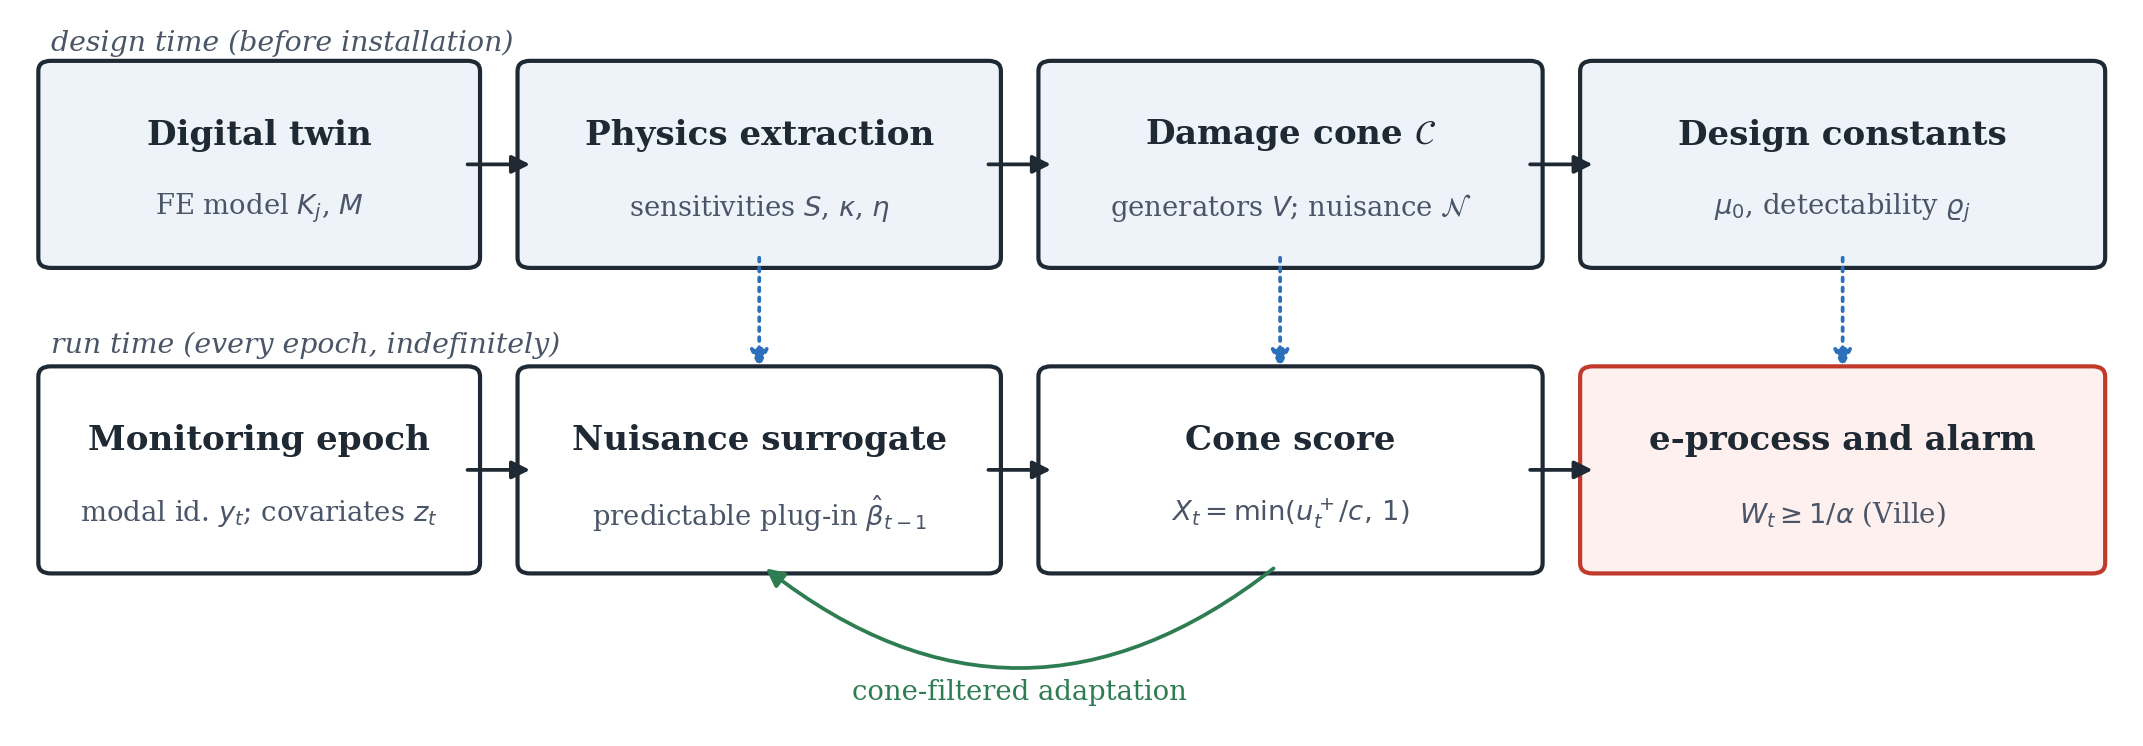
\includegraphics[width=\textwidth]{fig_pipeline.png}
\caption{The PHASE monitor. Quantities in the upper row are computed once, before installation, from the digital twin: the modal sensitivities, the damage cone and the nuisance subspace, and the design constants $\mu_0$ and the detectability map. The lower row runs at every interrogation epoch for the life of the installation. The feedback path is the identifiability-aware adaptation of Section~3.8, which allows the nuisance model to track drift while withholding residual components consistent with identifiable damage.}
\label{fig:pipeline}
\end{figure}

\subsection{Monitoring protocol and the anytime-valid decision problem}

A structure is interrogated at epochs $t=1,2,\dots$. At each epoch an automated operational modal analysis returns the first $m$ identified natural frequencies, collected as $y_t=\log \hat f_t\in\R^m$, together with measured covariates $z_t$ comprising ambient temperature deviation $\Delta T_t$ and a live-load proxy $q_t$. Let $\F_t=\sigma(y_1,z_1,\dots,y_t,z_t)$.

A commissioning window $t\le t_0$ is used to calibrate the monitor; monitoring proper runs for $t>t_0$ without a specified end. Write $H_0$ for the hypothesis that the structure remains in its reference condition throughout. A monitor is a stopping time $\tau$, the alarm time. The quantity of operational interest is
\begin{equation}
\mathrm{FWFA}(\alpha) \;=\; \Prob_{H_0}\!\left(\tau<\infty\right),
\label{eq:fwfa}
\end{equation}
the probability that the monitor \emph{ever} alarms on a healthy structure. We require $\mathrm{FWFA}\le\alpha$ for a horizon that is neither fixed nor known in advance. This is a strictly stronger requirement than per-epoch error control, and strictly stronger than average-run-length control, since it constrains the entire monitoring life rather than a rate.

\subsection{Physics: sensitivities, the damage cone, and the nuisance subspace}

Let $M$ be the mass matrix and $K(\theta)=\sum_{j=1}^{n}\theta_j K_j$ the stiffness matrix, with $K_j$ the contribution of substructure $j$ and $\theta_j$ a multiplier equal to one in the reference state. Writing $\lambda_i=\omega_i^2$ for the eigenvalues and $\phi_i$ for the mode shapes of $K\phi=\lambda M\phi$, first-order perturbation gives
\begin{equation}
\frac{\partial \lambda_i}{\partial \theta_j}=\frac{\phi_i^\top K_j \phi_i}{\phi_i^\top M \phi_i},
\qquad
S_{ij}:=\frac{\phi_i^\top K_j \phi_i}{\lambda_i\,\phi_i^\top M \phi_i}\ \ge 0 .
\label{eq:sens}
\end{equation}
Since $\log\omega_i=\tfrac12\log\lambda_i$, a stiffness loss $\rho_j=1-\theta_j\ge0$ at substructure $j$ shifts the log-frequencies by
\begin{equation}
\Delta \log \omega \;=\; -\tfrac{1}{2}\,S\rho + O(\|\rho\|^2).
\label{eq:shift}
\end{equation}
Two structural facts follow and are used throughout. First, $S$ is elementwise non-negative: stiffness loss can only lower frequencies. Second, because $K(\theta)$ is homogeneous of degree one in $\theta$, a uniform scaling $\theta=(1-\rho)\mathbf{1}$ scales all eigenvalues equally, whence
\begin{equation}
\textstyle\sum_{j} S_{ij}=1 \quad\text{for every mode } i .
\label{eq:rowsum}
\end{equation}

A uniform change in elastic modulus, which is how temperature principally acts, therefore shifts every log-frequency by the same amount. Writing $\kappa=S\mathbf{1}=\mathbf{1}$ for the uniform-modulus sensitivity and $\eta_i=\big(\sum_{k\in\mathcal{L}}\phi_{ik}^2 m_k\big)/(\phi_i^\top M\phi_i)$ for the sensitivity to relative added mass on loaded floors $\mathcal{L}$, the nuisance reaches the modal set only through the two directions $\kappa$ and $\eta$, whatever the functional form of the underlying EOV law.

Let $D=\mathrm{diag}(\sigma_1,\dots,\sigma_m)$ hold the identification scatter of each log-frequency and define standardised quantities $\tilde d_j=-D^{-1}S e_j$. The \emph{damage cone} is the finitely generated convex cone
\begin{equation}
\Cone=\Big\{-D^{-1}S\rho:\ \rho\in\R^n_{+}\Big\}
=\mathrm{cone}\{\tilde d_1,\dots,\tilde d_n\},
\label{eq:cone}
\end{equation}
which is pointed because all its generators lie in the negative orthant. The \emph{nuisance sensitivity subspace} is $\mathcal{N}=\mathrm{span}\{D^{-1}\kappa,\,D^{-1}\eta\}$, with orthogonal projector $P_\perp=I-\Pi_{\mathcal{N}}$.

\begin{proposition}[Identifiability]\label{prop:ident}
To first order, a stiffness-loss pattern $\rho$ produces a modal signature that is indistinguishable from some combination of a uniform modulus change and a live-load change if and only if $D^{-1}S\rho\in\mathcal{N}$. In particular, uniform stiffness loss $\rho\propto\mathbf{1}$ is always confounded with a temperature change. The identifiable part of the signature of $\rho$ is $P_\perp D^{-1}S\rho$, and monitoring of $n$ substructures requires $m>\dim\mathcal{N}=2$ identified modes.
\end{proposition}

The proof is immediate from \eqref{eq:rowsum} and is given in the Appendix. The practical content is considerable: no monitor, however sophisticated, can separate a global loss of stiffness from a warming of the structure using modal frequencies alone, and the ratio
\begin{equation}
\varrho_j \;=\; \frac{\|P_\perp \tilde d_j\|}{\|\tilde d_j\|}\ \in[0,1]
\label{eq:retention}
\end{equation}
gives a design-time \emph{detectability map} over the structure: the fraction of substructure $j$'s signature that survives confounding with the nuisance. Section~4.2.5 shows that this map is informative about localisation but, over practical horizons, not about detection, for reasons that are themselves instructive.


\subsection{Physics-structured nuisance surrogate with sequential plug-in}

The surrogate predicts reference-condition log-frequencies from covariates. Physics fixes its structure:
\begin{equation}
g_\beta(z_t)_i \;=\; a_i \;+\; b\,\kappa_i\,\Delta T_t \;+\; c\,\eta_i\, q_t ,
\qquad \beta=(a_1,\dots,a_m,b,c),
\label{eq:surrogate}
\end{equation}
with $\kappa_i$ and $\eta_i$ supplied by the digital twin through \eqref{eq:sens}. The model has $m+2$ free scalars; the temperature response is a single scalar shared across all modes, an exact consequence of \eqref{eq:rowsum}. The comparator used in the ablations is an unconstrained per-mode quadratic regression on $[1,\Delta T,\Delta T^2,q,\Delta T q]$ with $5m$ free parameters.

Coefficients are updated recursively with forgetting factor $\nu$, and crucially the prediction at epoch $t$ uses $\hat\beta_{t-1}$, estimated from data up to $t-1$ only. The standardised residual
\begin{equation}
r_t \;=\; D^{-1}\big(y_t-g_{\hat\beta_{t-1}}(z_t)\big)
\label{eq:resid}
\end{equation}
is thus a \emph{sequential plug-in} residual, and any statistic formed from $\hat\beta_{t-1}$ is $\F_{t-1}$-measurable. This predictability, not the accuracy of $\hat\beta$, is what preserves the martingale property in Section~3.5.

\subsection{Polyhedral approximation of the damage cone and the score}

For a closed convex cone, $\sup_{v\in\Cone,\|v\|\le1}\langle v,r\rangle=\|\Pi_\Cone(r)\|$. Rather than solving a non-negative least-squares projection at every epoch, PHASE fixes a finite set $V=\{v_1,\dots,v_N\}$ of unit vectors in $\Cone$ -- the normalised generators together with normalised pairwise combinations -- and scores
\begin{equation}
u_t=\max_{k\le N}\langle v_k,r_t\rangle,\qquad
X_t=\min\!\big(\max(u_t,0)/c,\,1\big)\in[0,1].
\label{eq:score}
\end{equation}
Evaluating \eqref{eq:score} is a single $N\times m$ matrix--vector product, which matters for edge deployment on a gateway alongside the sensor array.

\begin{proposition}[Polyhedral approximation]\label{prop:poly}
For every $r$, $\max_k\langle v_k,r\rangle\le\|\Pi_\Cone(r)\|$, and if $V$ has covering radius $\gamma$ in $\Cone\cap\mathbb{S}^{m-1}$ then $\max_k\langle v_k,r\rangle\ \ge\ \|\Pi_\Cone(r)\|-2\sin(\gamma/2)\,\|r\|$. The approximation is monotone: refining $V$ cannot decrease the score.
\end{proposition}

The null hypothesis is stated directly in terms of the score,
\begin{equation}
H_0:\quad \E[X_t\mid \F_{t-1}]\ \le\ \mu_0 \quad\text{for all } t,
\label{eq:null}
\end{equation}
where $\mu_0=\E_{\varepsilon\sim N(0,I_m)}\big[\min(\max_k\langle v_k,\varepsilon\rangle^+/c,1)\big]$ is a design-time constant obtained once by Monte Carlo from the digital twin. Stating the null this way is deliberate: it makes explicit that the surrogate's task is to render \eqref{eq:null} true in the reference condition, and Section~3.6 prices the failure to do so rather than assuming it away.

\subsection{Betting e-process and the alarm rule}

For $\lambda\in[0,1/\mu_0)$ define the wealth process $W_0^\lambda=1$ and
\begin{equation}
W_t^\lambda=\prod_{s=t_0+1}^{t}\big(1+\lambda(X_s-\mu_0)\big),
\qquad
W_t=\frac{1}{|\Lambda|}\sum_{\lambda\in\Lambda}W_t^\lambda ,
\label{eq:wealth}
\end{equation}
mixing over a fixed geometric grid $\Lambda$ so that no bet size need be tuned \citep{waudbysmith2024betting}. The alarm is
\begin{equation}
\tau=\inf\{t> t_0:\ W_t\ge 1/\alpha\}.
\label{eq:alarm}
\end{equation}

\begin{proposition}[Anytime validity]\label{prop:valid}
Under \eqref{eq:null}, $(W_t)_{t>t_0}$ is a non-negative supermartingale with $W_{t_0}=1$, and consequently $\Prob_{H_0}(\exists t: W_t\ge1/\alpha)\le\alpha$. The bound holds for arbitrary dependence in $(y_t,z_t)$, for any predictable bet sequence, for sequential plug-in estimation of $\hat\beta$, and irrespective of when or how often the operator inspects the process.
\end{proposition}

Two features deserve emphasis. First, no pre-change distribution need be known: only the conditional mean bound \eqref{eq:null} is required, and the score is bounded by construction, so no tail assumption enters. Second, $\log W_t$ is directly interpretable as accumulated evidence in nats, so an operator may act on a rising process before it crosses the threshold without invalidating anything -- the guarantee is uniform over stopping rules.

\subsection{Pricing surrogate misspecification}

Real EOV laws are never captured exactly. Thermal lag, vertical temperature gradients and imperfect load proxies leave a residual bias, so that \eqref{eq:null} holds only up to some $\delta\ge0$.

\begin{proposition}[Bias discount]\label{prop:delta}
Suppose $\E[X_t\mid\F_{t-1}]\le\mu_0+\delta$ for all $t$. Then
$\widetilde W^\lambda_t = W^\lambda_t/(1+\lambda\delta)^{t-t_0}$
is a non-negative supermartingale, and the alarm rule \eqref{eq:alarm} applied to the mixture of $\widetilde W^\lambda$ satisfies $\mathrm{FWFA}\le\alpha$.
\end{proposition}

PHASE estimates $\delta$ from the second half of the commissioning window as an upper confidence limit on the excess score, $\hat\delta=(\bar X-\mu_0+2\,\widehat{\mathrm{se}})^{+}$, and discounts the evidence at $\log(1+\lambda\hat\delta)$ nats per epoch. This converts model quality into a currency: a surrogate that leaves half the bias buys back half the discount, and the mechanism gives a precise sense in which better physics is worth more than better statistics.

\subsection{Detection delay}

\begin{proposition}[Delay bound]\label{prop:delay}
Suppose that after change point $t^\star$ the score satisfies $\E[\log(1+\lambda(X_t-\mu_0))\mid\F_{t-1}]\ge g(\lambda)>\log(1+\lambda\delta)$ for some $\lambda\in\Lambda$. Then the alarm time satisfies
\begin{equation}
\E[\tau-t^\star]\ \le\ \frac{\log(1/\alpha)+\log|\Lambda|+B+(\log W_{t^\star})^{-}}{g(\lambda)-\log(1+\lambda\delta)},
\label{eq:delay}
\end{equation}
where $B$ bounds the increment overshoot.
\end{proposition}

The bound has the expected shape: delay grows logarithmically in $1/\alpha$ and inversely in the evidence growth rate, and the bias discount subtracts directly from that rate. Restricting the alternative to the cone raises $g(\lambda)$ by removing the noise that an omnibus statistic must accumulate over all directions, which is why the cone ablation in Section~4 loses so much power.

\subsection{Identifiability-aware adaptation}

Online adaptation of a nuisance model in a damage detector is dangerous: with forgetting factor $\nu$, the surrogate absorbs a persistent step within roughly $1/(1-\nu)$ epochs, and a detector whose reference model chases the damage will eventually go quiet. Freezing the surrogate after commissioning avoids this but forfeits tracking of genuine long-term drift, and in preliminary experiments a naive evidence-gated freeze produced a positive feedback loop in which a frozen surrogate generated ever-larger residuals.

Physics resolves the tension. Let $\tilde V$ denote the generators of the cone projected onto $\mathcal{N}^\perp$ and normalised, and let $w_t=\max_k\langle\tilde v_k,r_t\rangle^{+}\,\tilde v_{k^\star}$ be the identifiable damage-consistent component of the residual. The surrogate is updated towards the target
\begin{equation}
y_t - D\big(r_t-\mathrm{clip}(r_t-w_t,\pm\varsigma)\big),
\label{eq:filtered}
\end{equation}
that is, the identifiable damage-consistent component is withheld from adaptation while everything else, Huber-clipped at $\varsigma$, is retained. Because the nuisance acts within $\mathcal{N}$ and the withheld component lies in $\mathcal{N}^\perp$, the surrogate remains free to learn the entire temperature and live-load response -- which it must, since temperature acts inside the damage cone -- while identifiable damage cannot be absorbed. The rule is a fixed function of $r_t$ and so preserves predictability.

\subsection{Localisation and multiple zones}

The generator attaining the maximum in \eqref{eq:score} carries a support over substructures. Accumulating $L_j \mathrel{+}= \mathrm{supp}_j(v_{k^\star})\,(X_t-\mu_0)^{+}$ over the monitoring period yields a localisation index whose argmax names the implicated substructure. For structures partitioned into zones, a separate e-process per zone can be run and the zone-level processes merged by averaging, which is valid under arbitrary dependence \citep{vovk2021evalues}; if zone-level claims are wanted, e-values support false discovery rate control directly \citep{wang2022fdr}, avoiding the conservatism of a Bonferroni correction across zones.

\begin{algorithm}[t]
\caption{PHASE monitoring cycle (one epoch)}
\begin{algorithmic}[1]
\State \textbf{Design time:} $S,\kappa,\eta$ from the twin; generators $V,\tilde V$; projector $P_\perp$; $\mu_0$ by Monte Carlo
\State \textbf{Commissioning:} fit $\hat\beta$; estimate $D$; estimate $\hat\delta$ on held-out commissioning epochs
\For{$t>t_0$}
  \State $r_t \gets D^{-1}(y_t-g_{\hat\beta_{t-1}}(z_t))$ \Comment{sequential plug-in}
  \State $u_t\gets\max_k\langle v_k,r_t\rangle$; \ $X_t\gets\min(u_t^{+}/c,1)$
  \State $\log W^\lambda_t \gets \log W^\lambda_{t-1}+\log(1+\lambda(X_t-\mu_0))-\log(1+\lambda\hat\delta)$ for $\lambda\in\Lambda$
  \State \textbf{if} $\mathrm{logmeanexp}_\lambda \log W^\lambda_t\ \ge\ \log(1/\alpha)$ \textbf{then} raise alarm; report localisation index
  \State update $\hat\beta$ towards the cone-filtered target \eqref{eq:filtered}
\EndFor
\end{algorithmic}
\end{algorithm}

\section{Simulation study}

\subsection{Experimental design}

\subsubsection{Digital twin and data generation}

The test structure, drawn in Figure~\ref{fig:frame}, is an eight-storey shear frame with storey mass $2.5\times10^5$\,kg and storey stiffness $6.0\times10^{8}$\,N/m, giving reference frequencies of 1.44, 4.27, 6.95, 9.40, 11.52 and 13.26\,Hz for the $m=6$ identified modes. Epochs are six hours apart, corresponding to automated modal identification four times per day, and records span two years (2{,}920 epochs) with a one-year commissioning window unless stated otherwise.


\begin{figure}[t]
\centering
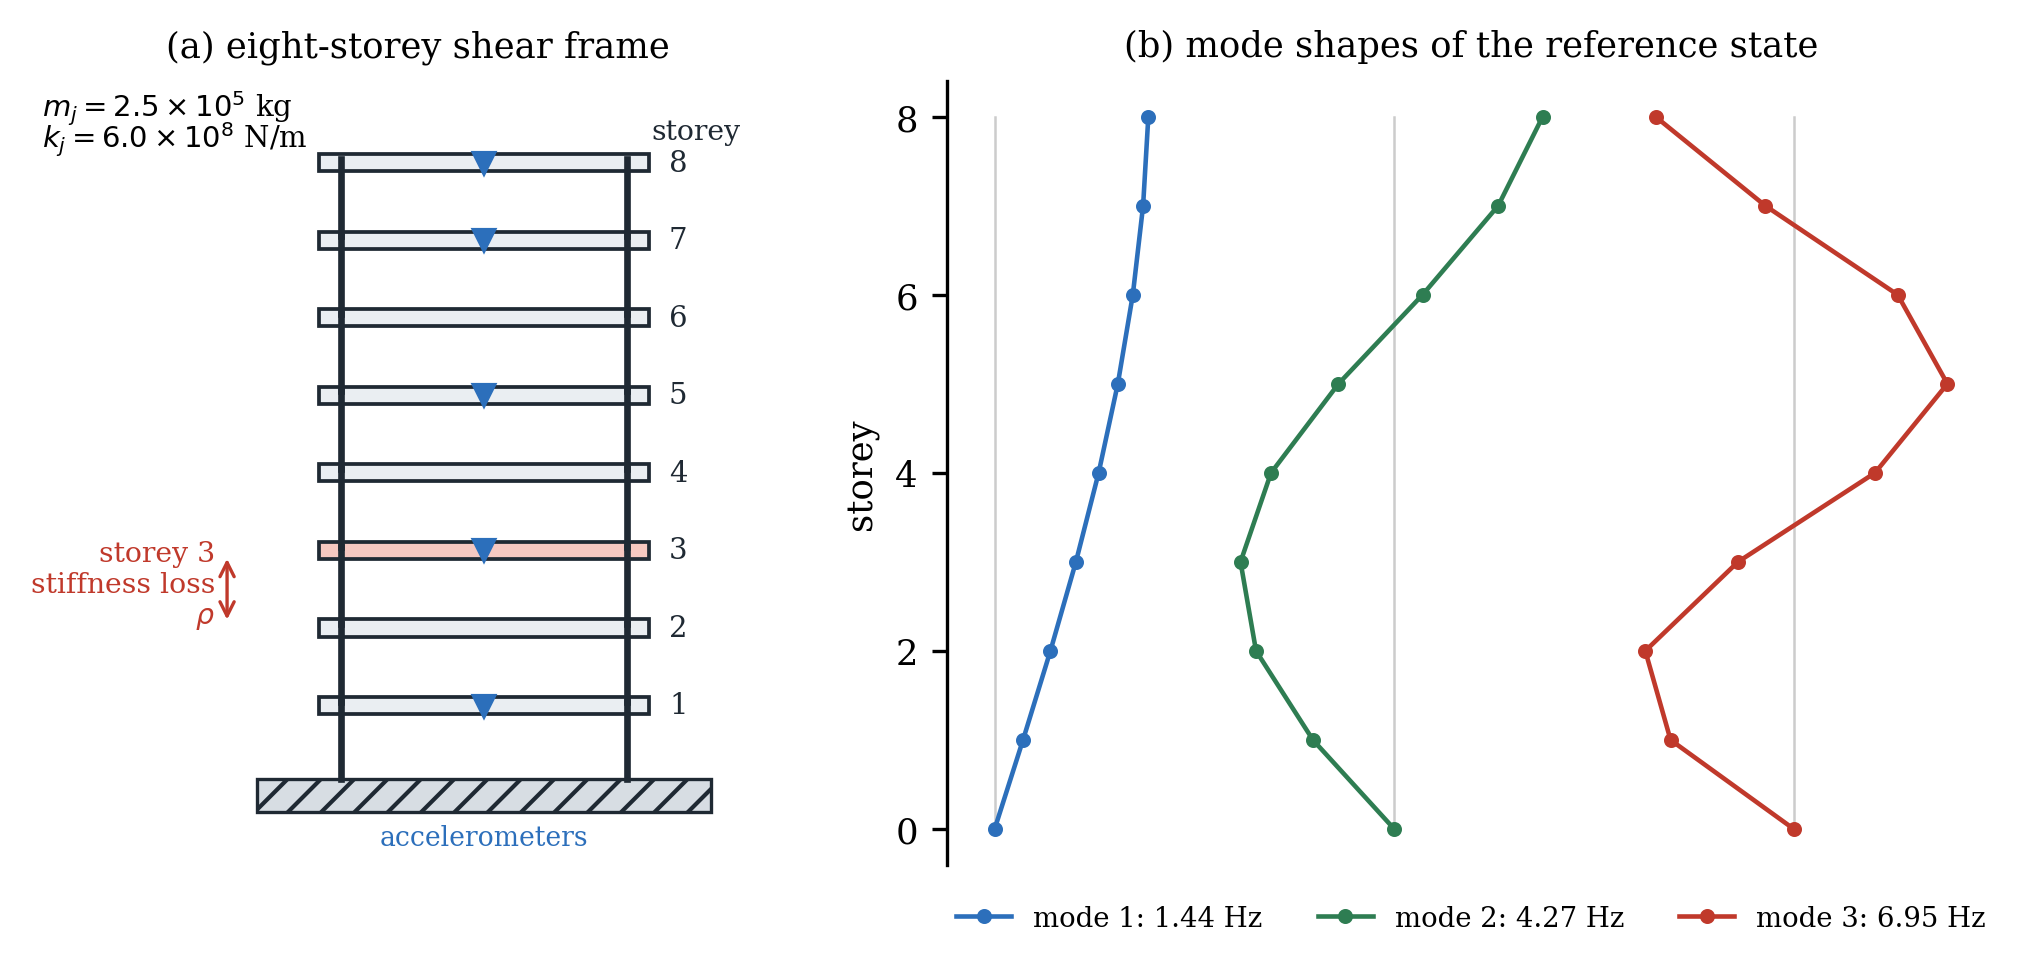
\includegraphics[width=\textwidth]{fig_frame.png}
\caption{The simulated structure. (a) Eight-storey shear frame with lumped storey masses and storey stiffnesses; damage is introduced as a multiplicative stiffness loss at a single storey, storey~3 unless stated otherwise. (b) Mode shapes and natural frequencies of the reference state, from which the sensitivity matrix $S$ of equation~\eqref{eq:sens} is computed.}
\label{fig:frame}
\end{figure}

Environmental forcing follows a northern-Vietnam monsoon calendar: an annual temperature cycle of $24\pm7^\circ$C, a diurnal cycle of amplitude $4^\circ$C, and autocorrelated weather noise, giving an ambient range of roughly $10$--$39^\circ$C. Three features are deliberately \emph{not} available to the monitor. Storey temperatures follow ambient through first-order thermal lags with storey-dependent time constants and a vertical gradient spanning $\pm15\%$; the live load acts on floors 2--7 with an occupancy and weekday cycle and is observed only through a proxy with 10\% multiplicative error; and modal identification noise is Student-$t$ with five degrees of freedom, scaled to 0.60--1.20\% relative standard deviation across modes. The monitor sees only single-sensor ambient temperature and the load proxy, so its surrogate is misspecified in exactly the way field surrogates are.

Modulus depends on temperature with $\beta_T=2.5\times10^{-3}$\,$^\circ$C$^{-1}$. Frequencies are computed exactly by solving the generalised eigenproblem at each epoch, not by the perturbation formula used by the monitor, so the first-order model is genuinely approximate from the monitor's point of view.

\subsubsection{Scenarios}

Seven scenarios are simulated, each with damage onset at epoch 1{,}825 (year 1.25) where applicable: abrupt stiffness loss of 2\%, 5\% and 10\% at storey 3; a gradual loss reaching 6\% at storey 3 over 60 days; abrupt 5\% loss at storeys 1 and 6, chosen for their contrasting identifiable fractions; a benign 3\% \emph{stiffening} of all storeys, representing temporary propping during façade works, which must not trigger a damage alarm; and undamaged records. Undamaged records are also simulated over four years to test behaviour beyond a calibration horizon.

\subsubsection{Comparators}

All comparators consume the same residual stream where possible, so that differences reflect the decision rule rather than the features. \textbf{PHASE} is the full method. \textbf{PHASE (no discount)} omits Proposition~\ref{prop:delta}. \textbf{PHASE-$\Omega$} replaces the cone score with the omnibus norm $\|r_t\|$, retaining all other machinery. \textbf{PHASE-BB} replaces the physics-structured surrogate with the unconstrained per-mode regression. \textbf{PHASE-E} additionally suspends betting when covariates fall outside the commissioning envelope.

Four comparators represent current SHM practice. The \textbf{$3\sigma$ chart} alarms when any $|r_{it}|>3$. The \textbf{calibrated chart} uses a threshold set at the 99th percentile of the healthy maximum over a one-year monitoring horizon, obtained from 150 independent healthy simulations. The \textbf{Mahalanobis novelty index} is the classical outlier statistic $\sqrt{r_t^\top\hat\Sigma^{-1}r_t}$ with a threshold calibrated the same way rather than taken from a $\chi^2$ table. The \textbf{PCA-EOV chart} implements the standard data-normalisation strategy directly: the leading two principal components of the commissioning log-frequency matrix, which are dominated by environmental response, are projected out and the norm in the retained subspace is charted, again with a simulation-calibrated threshold. The \textbf{repeated $T^2$ test} applies a $\chi^2_m$ test at the 1\% level every epoch.

Three comparators represent classical sequential detection, all applied to the same cone score and all with thresholds calibrated to a one-year horizon on 150 healthy simulations: \textbf{CUSUM}, the \textbf{Shiryaev--Roberts} procedure, and an \textbf{EWMA} chart. These are oracles in a strong sense, since they require 150 replicated realisations of the true healthy process, which no real deployment possesses.

Finally, the \textbf{conformal test martingale} is an anytime-valid comparator that obtains its guarantee differently from PHASE. Cone scores from the commissioning window serve as a calibration set; each monitoring epoch yields a smoothed conformal $p$-value, and a mixture of power martingales $\int_0^1\prod_s \epsilon p_s^{\epsilon-1}\,\mathrm{d}\epsilon$ accumulates evidence, with the same Ville alarm at $1/\alpha$ \citep{vovk2021testing}. It uses the identical score and the identical alarm rule, so the comparison isolates one question: whether validity should rest on exchangeability of the calibration sample or, as in PHASE, on a conditional mean bound with an explicit misspecification discount.

\subsubsection{Metrics}

We report the family-wise false-alarm probability \eqref{eq:fwfa} over one- and three-year monitoring horizons; detection rate and detection delay after onset; pre-onset false alarms in damage scenarios; and localisation accuracy. All rates are reported with standard errors. In total 2{,}700 records were simulated: 150 for threshold calibration, 300 healthy over two years, 300 healthy over four years, 150 per damage scenario, and 800 across the commissioning sweep.

\subsection{Results}

\subsubsection{Validity of the first-order physics}

Table~\ref{tab:validation} compares the exact log-frequency shift from re-solving the eigenproblem with the first-order prediction $-\tfrac12 S\rho$. At 2\% stiffness loss the maximum relative error across modes is below 1.9\%, rising to 9.3\% at 10\% loss. The perturbation basis on which the cone and the sensitivity structure rest is therefore accurate over the damage range of interest, with the approximation degrading gracefully and conservatively.

\begin{table}[t]
\centering
\small
\caption{Accuracy of the first-order sensitivity model against exact eigen-solution. Relative error is the maximum across the six identified modes.}
\label{tab:validation}
\begin{tabular}{lccc}
\toprule
Stiffness loss & Storey 1 & Storey 3 & Storey 6 \\
\midrule
2\%  & 1.9\% & 1.7\% & 1.8\% \\
5\%  & 4.6\% & 4.2\% & 4.6\% \\
10\% & 9.3\% & 8.2\% & 9.2\% \\
\bottomrule
\end{tabular}
\end{table}

\subsubsection{False-alarm control under continuous monitoring}

Table~\ref{tab:fwer} reports the probability that each monitor ever alarms on an undamaged structure. The $3\sigma$ chart and the repeated $T^2$ test alarmed in every record, at median elapsed times of 2.0 and 3.5 days respectively. This is the expected consequence of applying a fixed-sample rule 1{,}460 times, and it is the behaviour that drives alarm fatigue in deployed systems.

\begin{table}[t]
\centering
\small
\caption{Family-wise false-alarm probability on undamaged structures (standard errors in parentheses). One-year results from 300 two-year records; three-year results from 300 four-year records. The calibrated chart and CUSUM thresholds were tuned for a one-year monitoring horizon.}
\label{tab:fwer}
\begin{tabular}{lcc}
\toprule
Monitor & 1-year horizon & 3-year horizon \\
\midrule
\multicolumn{3}{l}{\textit{anytime-valid by construction}}\\
PHASE & \textbf{0.000} (0.000) & \textbf{0.000} (0.000) \\
PHASE-E (envelope gated) & 0.000 (0.000) & 0.000 (0.000) \\
PHASE-$\Omega$ (no cone) & 0.000 (0.000) & 0.000 (0.000) \\
PHASE-BB (black-box surrogate) & 0.000 (0.000) & 0.000 (0.000) \\
PHASE, no bias discount & 0.003 (0.003) & 0.017 (0.007) \\
Conformal test martingale & 0.033 (0.010) & 0.030 (0.010) \\
\midrule
\multicolumn{3}{l}{\textit{sequential detection, horizon-calibrated oracles}}\\
CUSUM & 0.003 (0.003) & 0.000 (0.000) \\
Shiryaev--Roberts & 0.003 (0.003) & 0.000 (0.000) \\
EWMA & 0.003 (0.003) & 0.020 (0.008) \\
\midrule
\multicolumn{3}{l}{\textit{current SHM practice}}\\
Calibrated chart (oracle) & 0.007 (0.005) & 0.023 (0.009) \\
Mahalanobis novelty index & 0.007 (0.005) & 0.023 (0.009) \\
PCA-EOV chart & 0.017 (0.007) & 0.040 (0.011) \\
$3\sigma$ chart & 1.000 & 1.000 \\
Repeated $T^2$ test & 1.000 & 1.000 \\
\midrule
\multicolumn{3}{l}{\footnotesize Nominal level $\alpha=0.01$.} \\
\bottomrule
\end{tabular}
\end{table}

The more interesting comparisons are with the methods that do control error to some degree. Given 150 replications of the true healthy process, the oracle-calibrated chart holds to 0.007 over the horizon for which it was tuned, but its false-alarm probability then grows without bound as monitoring continues, reaching 0.023 at three years and still rising (Figure~\ref{fig:fwer}). The Mahalanobis novelty index behaves identically, and the PCA-EOV chart -- the closest comparator to standard data-normalisation practice -- is worse at both horizons, at 0.017 and 0.040. The distinction is not a matter of a better-chosen threshold: a threshold calibrated for a horizon is valid only at that horizon, whereas a supermartingale threshold is valid at all of them simultaneously.

The conformal test martingale is the most informative comparator, because it is anytime-valid by construction and yet exceeded the nominal level, at 0.033 and 0.030. Ville's inequality is not at fault; the exchangeability assumption is. Conformal calibration treats the commissioning scores and the monitoring scores as exchangeable, and slow environmental drift breaks that assumption in a way that inflates evidence steadily rather than sporadically. PHASE makes no exchangeability assumption. It requires only the conditional mean bound \eqref{eq:null}, and prices the failure of that bound through $\hat\delta$. The comparison isolates the ingredient: given the same score and the same alarm rule, the conditional-mean formulation with an explicit misspecification discount controls error where distribution-free conformal calibration does not.

The value of the bias discount is visible in the same table. Without it, PHASE's false-alarm probability was 0.003 at one year and 0.017 at three, exceeding the nominal level as the unmodelled thermal lag and gradient accumulated evidence at a slow but non-zero rate. With $\hat\delta$ estimated from commissioning data (mean 0.020, sd 0.011 across records), the excess was absorbed and no false alarm occurred in 600 healthy records totalling roughly 1{,}300 structure-years of monitoring.

\begin{figure}[t]
\centering
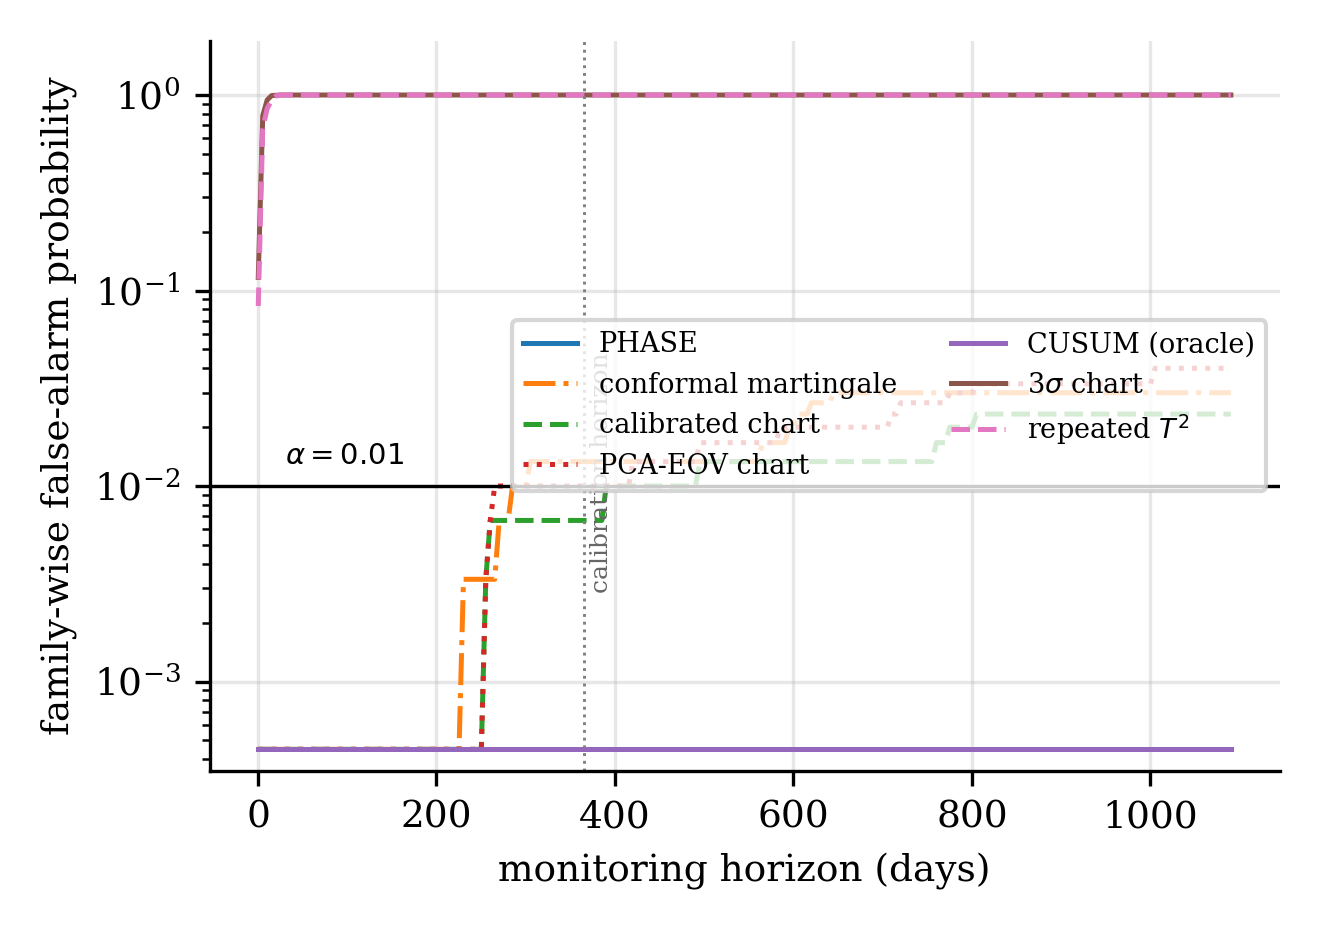
\includegraphics[width=0.72\textwidth]{fig_fwer.png}
\caption{Family-wise false-alarm probability as a function of monitoring horizon, from 300 undamaged four-year records. Curves for PHASE, PHASE-BB and the oracle CUSUM lie on the axis floor (no false alarm observed). The calibrated chart controls error only up to the horizon for which it was tuned.}
\label{fig:fwer}
\end{figure}

\subsubsection{Detection delay, localisation, and the cost of validity}

Table~\ref{tab:delay} reports detection performance. PHASE detected 5\% stiffness loss at storey 3 in every record with a median delay of 235 epochs (59 days, interquartile range 51--69 days), and 10\% loss with a median delay of 26 days. At 2\% loss -- a signature amounting to roughly 0.2\% frequency change against 0.6--1.2\% identification scatter -- detection within the remaining nine months occurred in 34\% of records. Gradual degradation reaching 6\% over 60 days was detected in every record, with a median delay of 80 days from onset of degradation.

\begin{table}[t]
\centering
\small
\caption{Detection rate within the remaining nine months of monitoring and median detection delay in days (interquartile range). All entries from 150 records per scenario. Localisation accuracy refers to PHASE.}
\label{tab:delay}
\setlength{\tabcolsep}{5pt}
\begin{tabular}{lcccccc}
\toprule
Scenario & PHASE & PHASE-$\Omega$ & PHASE-BB & Conformal & CUSUM & Loc. \\
\midrule
2\% storey 3   & 0.34 / 156 & 0.00 / ---  & 0.43 / 142 & 0.79 / 121 & 0.91 / 96 & 0.89 \\
5\% storey 3   & 1.00 / 59  & 0.29 / 157  & 1.00 / 57  & 1.00 / 45  & 1.00 / 26 & 1.00 \\
10\% storey 3  & 1.00 / 26  & 0.99 / 34   & 1.00 / 25  & 1.00 / 16  & 1.00 / 10 & 1.00 \\
Gradual 6\%    & 1.00 / 80  & 0.44 / 179  & 1.00 / 77  & 1.00 / 66  & 1.00 / 53 & 1.00 \\
5\% storey 1   & 1.00 / 38  & 0.60 / 108  & 1.00 / 37  & 1.00 / 28  & 1.00 / 16 & 0.00 \\
5\% storey 6   & 1.00 / 62  & 0.22 / 140  & 1.00 / 60  & 1.00 / 48  & 1.00 / 28 & 1.00 \\
\midrule
Benign stiffening & \textbf{0.00} & \textbf{1.00} / 11 & \textbf{0.00} & \textbf{0.00} & \textbf{0.00} & --- \\
\midrule
\multicolumn{7}{l}{\footnotesize PCA-EOV chart and Mahalanobis index: detection rate $\le 0.01$ in every damage scenario.}\\
\bottomrule
\end{tabular}
\end{table}

The results describe a frontier rather than a winner, and the costs of validity should be stated plainly. Every method that detects faster than PHASE pays for it somewhere. The oracle CUSUM and Shiryaev--Roberts procedures detect roughly twice as fast throughout and hold their error rate, but they are calibrated from 150 replications of the true healthy process and their guarantee is an average run length rather than a probability over the monitoring life; neither is available to a real deployment. The EWMA chart is faster still, at a median of 10 days for 5\% damage, but its false-alarm probability reaches 0.020 by three years and it detects only 17\% of 2\% losses. The conformal martingale detects 5\% damage in 45 days against PHASE's 59, and 79\% of 2\% losses against PHASE's 34\%, but at three times the nominal false-alarm rate. PHASE is the only method in the comparison with zero observed false alarms at both horizons that still detects every loss of 5\% or more.

The discount is part of that price: undiscounted PHASE detects 5\% loss in 43 days rather than 59, and 95\% of 2\% losses rather than 34\%, while drifting above the nominal level. Proposition~\ref{prop:delay} makes the exchange rate explicit.

At the other end of the frontier sit the two data-normalisation comparators. The PCA-EOV chart and the Mahalanobis index detected at most 1\% of damage in every scenario while also failing to control error beyond their calibration horizon -- the worst of both, and a caution against reading a quiet chart as a well-behaved monitor.

Two further observations concern the stiffening scenario. The EWMA, CUSUM, Shiryaev--Roberts and conformal comparators all remained silent there, but this is inherited rather than earned: each consumes the physics-derived cone score, and the directional restriction is what discards the change. Only PHASE-$\Omega$, which sees the omnibus norm, alarms. The physics, not the sequential machinery, supplies the discrimination.

The horizon-calibrated chart illustrates the opposite failure. Its threshold had to reach 24.3 standardised units to survive the EOV-contaminated residual stream, and it consequently detected 5\% damage in none of 150 records and 10\% damage in 1.3\%. Controlling false alarms by raising a threshold, rather than by accumulating evidence, sacrifices essentially all of the detection capability the monitoring system was installed to provide. Figure~\ref{fig:delay} summarises the severity--delay relationship for all variants.

\begin{figure}[t]
\centering
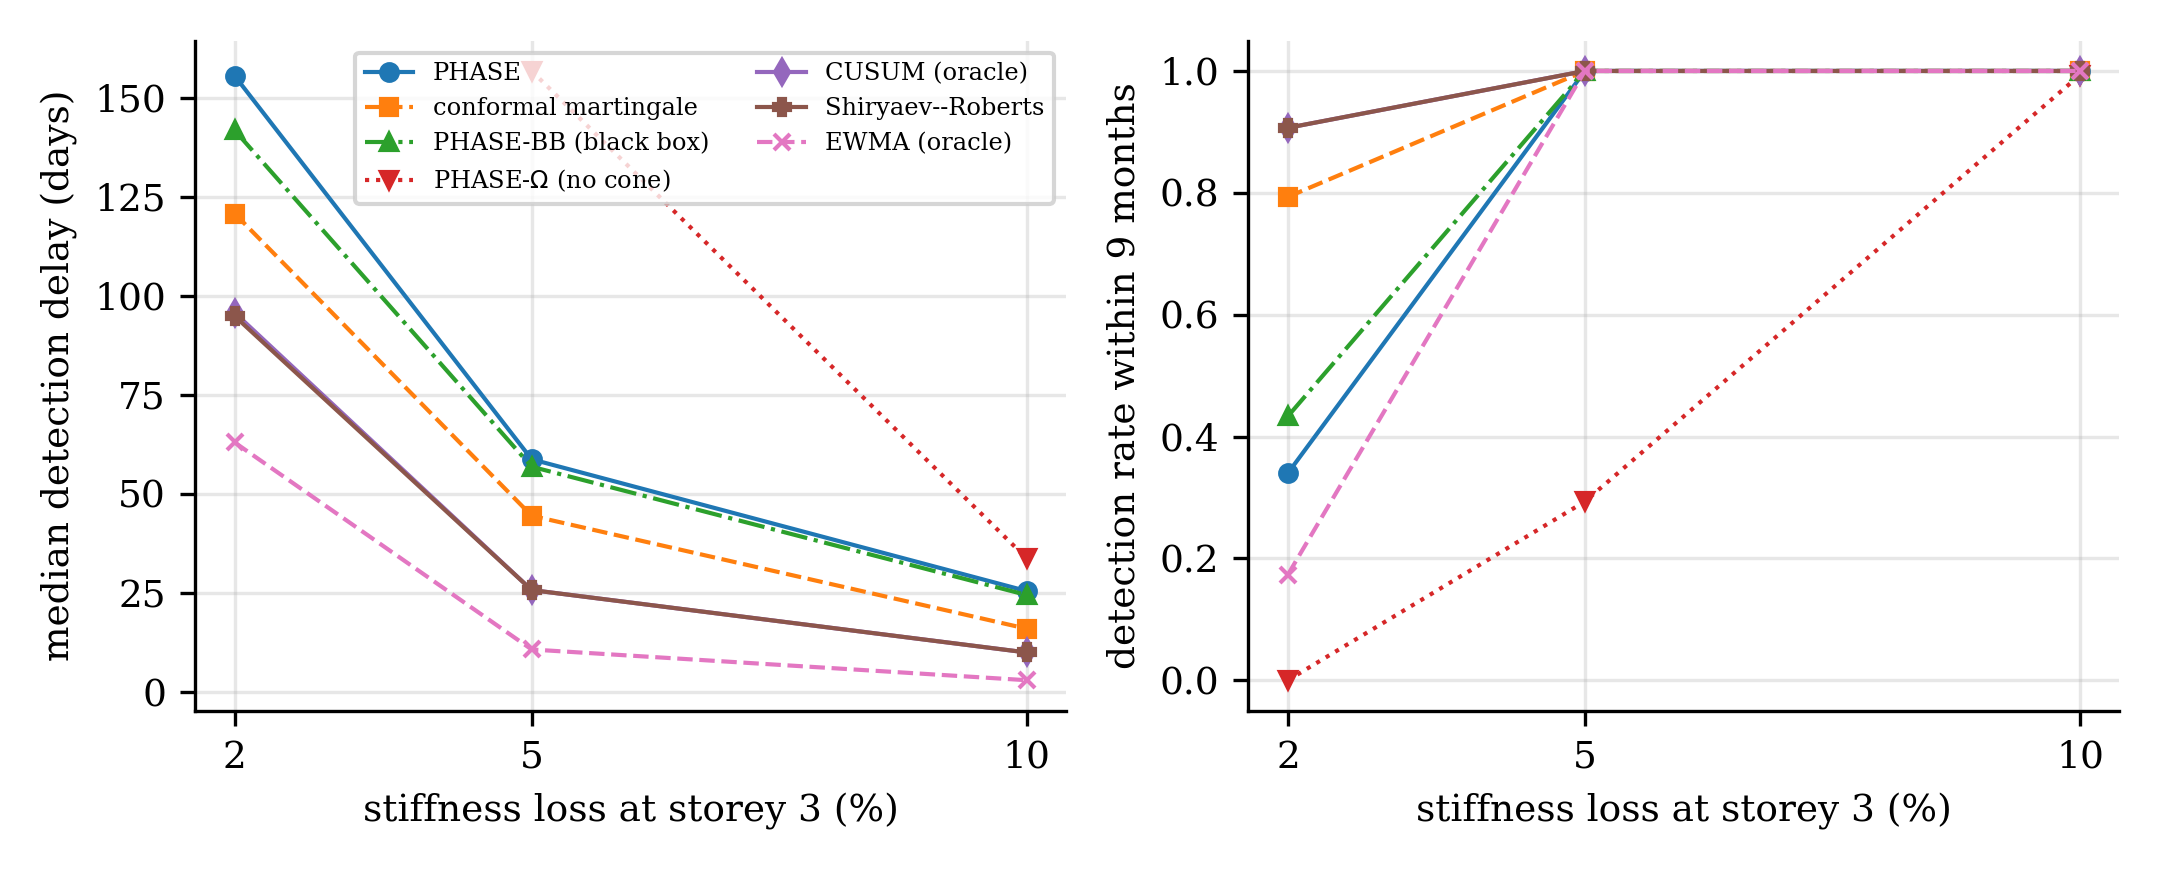
\includegraphics[width=\textwidth]{fig_delay.png}
\caption{Median detection delay (left) and detection rate within the remaining nine months (right) against damage severity at storey 3. The oracle CUSUM is faster throughout; the cone-free ablation loses most of the power.}
\label{fig:delay}
\end{figure}

\begin{figure}[t]
\centering
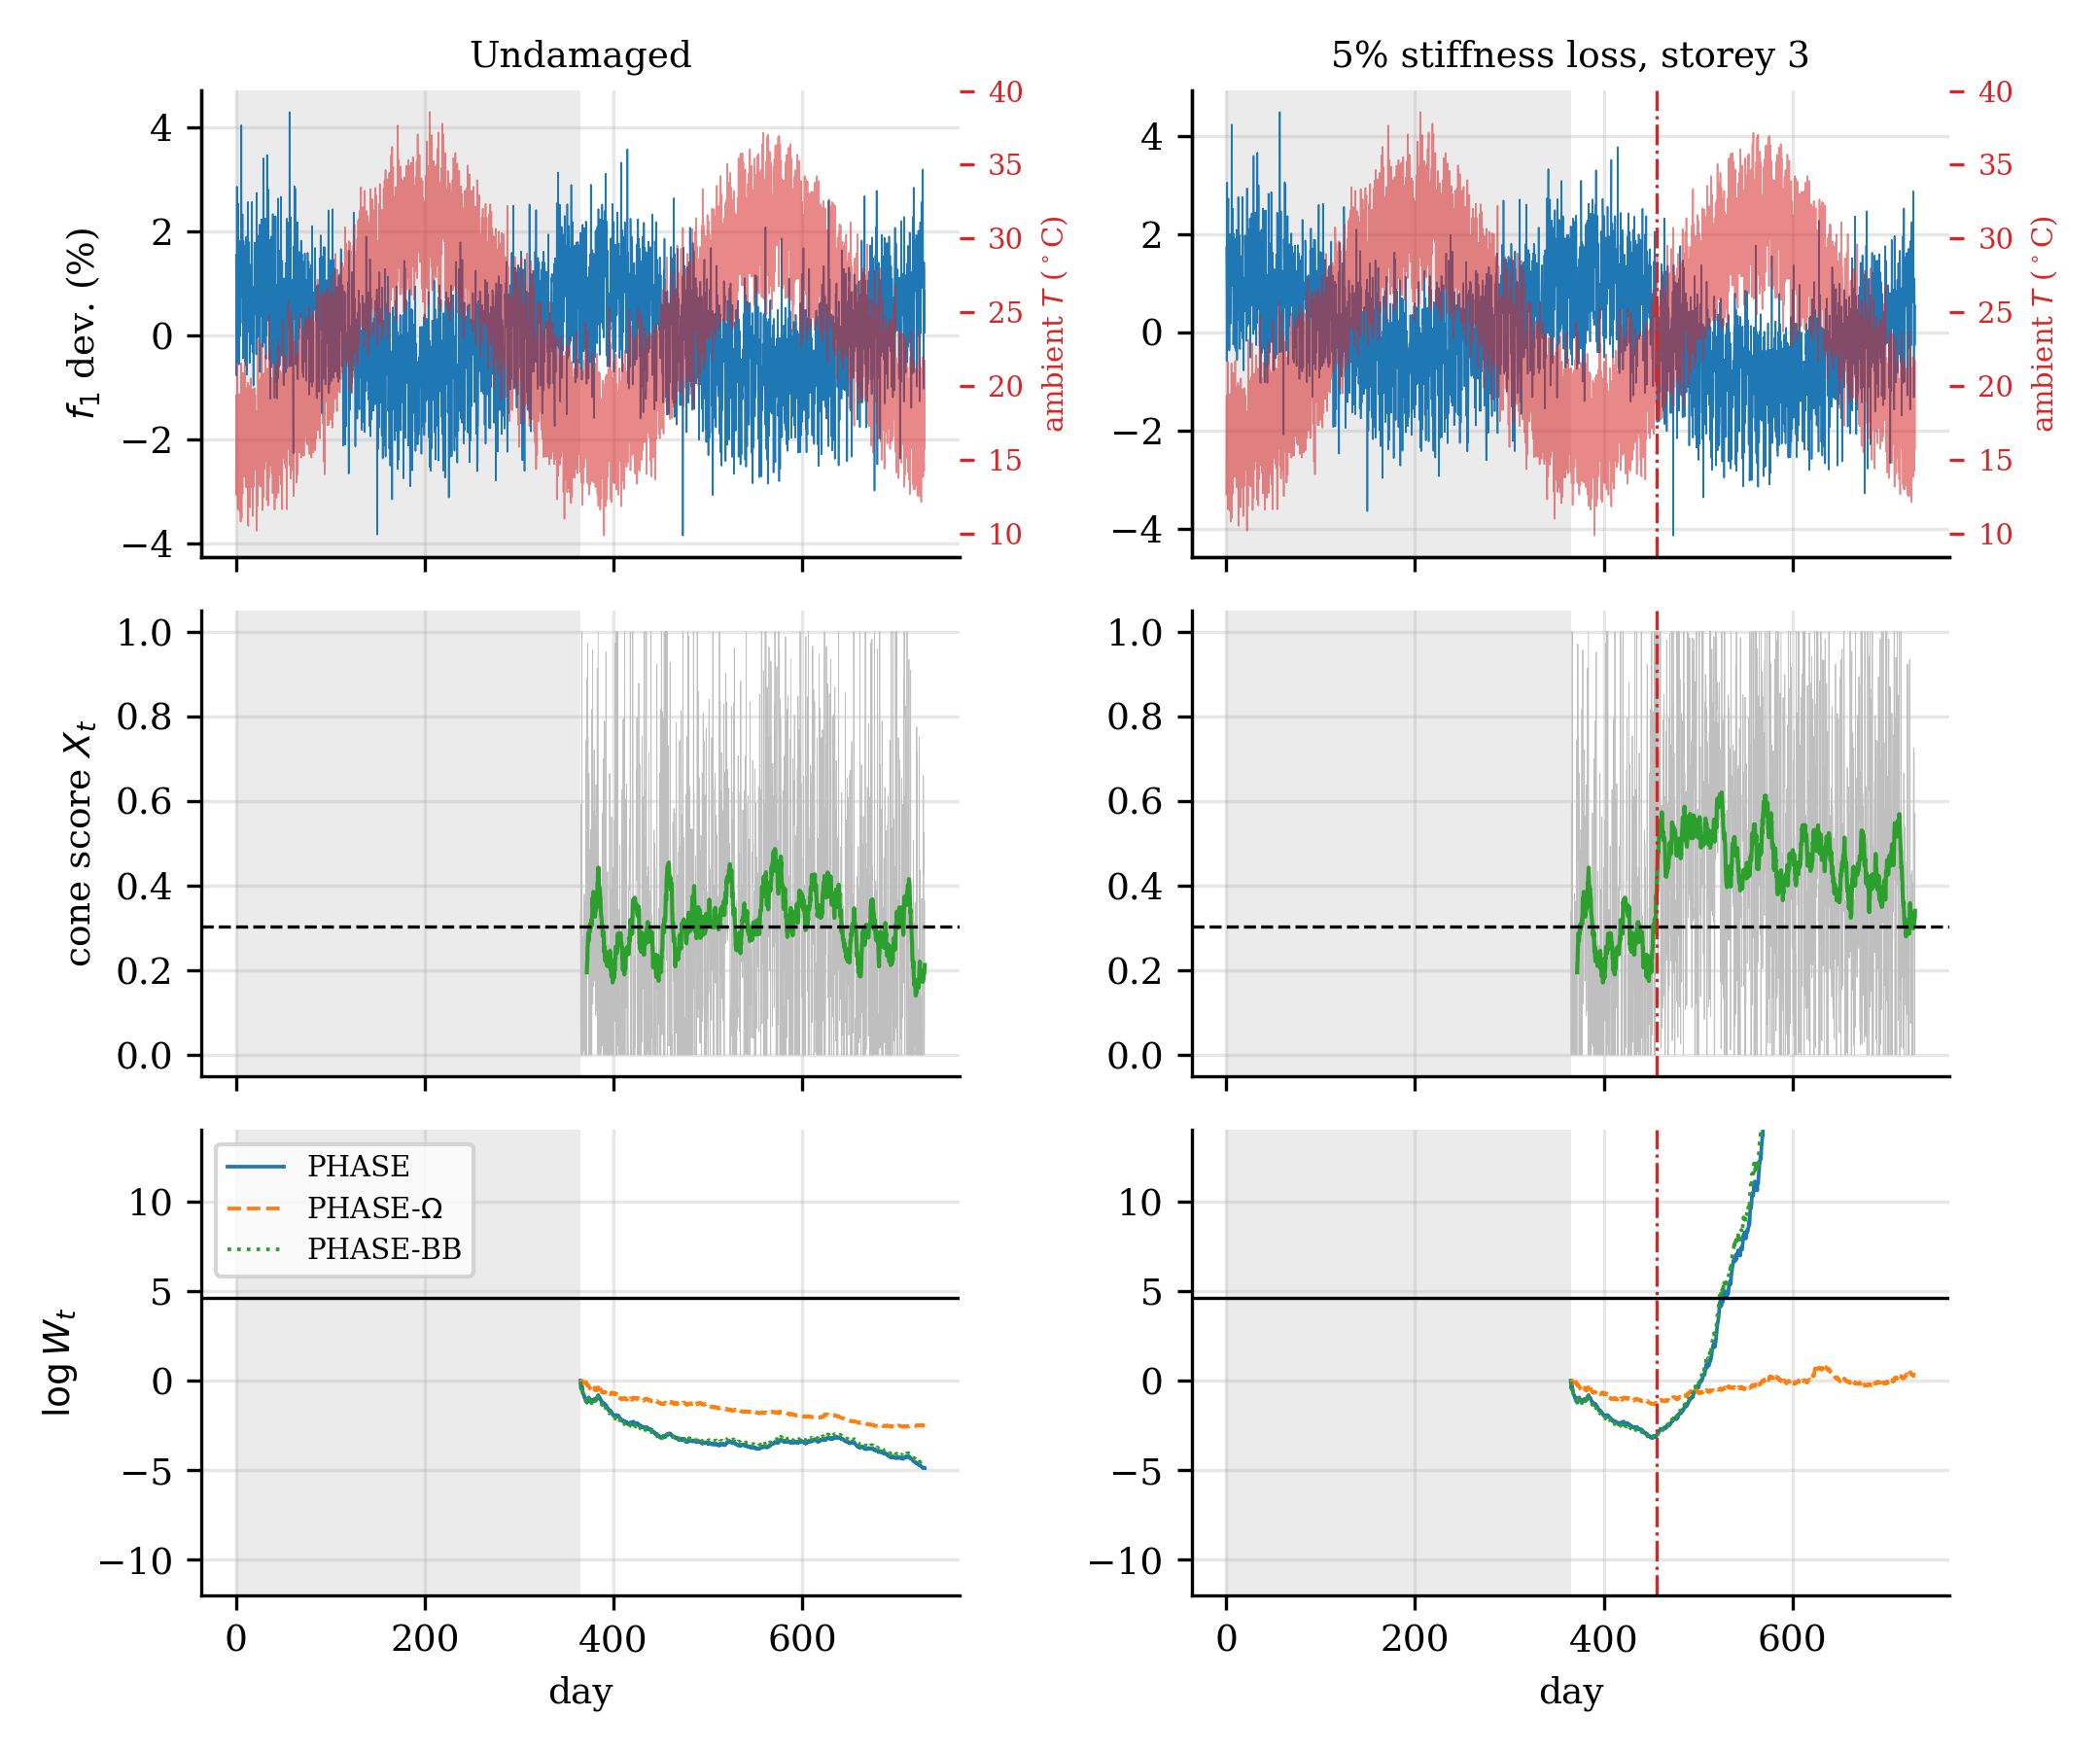
\includegraphics[width=\textwidth]{fig_records.png}
\caption{One undamaged (left) and one damaged (right) record. Top: fundamental-frequency deviation (blue) against ambient temperature (red); environmental variation exceeds the damage signature. Middle: cone score with 7-day mean and null mean $\mu_0$ (dashed). Bottom: accumulated log-evidence for PHASE and two ablations, with the alarm threshold $\log(1/\alpha)$. Shading marks commissioning; the dash-dotted line marks damage onset.}
\label{fig:records}
\end{figure}

\subsubsection{Discriminating benign change: the value of the damage cone}

The clearest single result concerns the stiffening scenario, in which temporary propping raises all storey stiffnesses by 3\%. This is a real change in the structure, and any omnibus change detector should and does find it: PHASE-$\Omega$ alarmed in all 150 records, at a median of 11 days. PHASE alarmed in none, because the change lies outside the damage cone -- frequencies rose, and stiffness loss cannot raise frequencies. The oracle CUSUM, which in our implementation consumes the same cone score, also correctly stayed silent, which underlines that the discriminating ingredient is the physics-derived restriction of the alternative and not the sequential machinery.

The cone contributes power as well as specificity. Removing it while holding everything else fixed reduced the detection rate for 5\% damage from 1.00 to 0.29 and roughly tripled the median delay (Table~\ref{tab:delay}). An omnibus statistic must accumulate noise over all $m$ directions; the cone restricts attention to the ones damage can actually produce.

\subsubsection{The detectability map: what physics can and cannot promise}

Figure~\ref{fig:detect} shows the identifiable fraction \eqref{eq:retention} for each storey. It ranges from 0.245 at storey 1 to 0.588 at storey 6: between 41\% and 76\% of each storey's modal signature is confounded with the nuisance directions and is unavailable for inference, however long one monitors.

The map's empirical content is more subtle than we anticipated, and the discrepancy is worth reporting. Detection delay did \emph{not} follow the identifiable fraction: 5\% loss at storey 1, whose identifiable fraction is lowest, was detected fastest (median 38 days) because its \emph{total} signature norm is largest (57.5 versus 42.2 standardised units for storey 3). The resolution is that the surrogate absorbs the confounded component only over its adaptation timescale, roughly 2{,}000 epochs here, which is longer than the detection delays observed. Over practical horizons detection is therefore governed by the full signature; the identifiable fraction governs the asymptotic regime.

Localisation, by contrast, follows the map exactly. Damage at storeys 3 and 6 was localised correctly in 150 of 150 records each. Damage at storey 1 was localised correctly in none: it was attributed to storey 3 in 75 records and storey 6 in 55, precisely the storeys whose identifiable directions best match the residual once the confounded component is removed. Detection and localisation are distinct capabilities, and the map predicts the second. For asset managers this is directly actionable: it states, before any sensor is installed, which substructures a proposed modal set can support claims about.

\begin{figure}[t]
\centering
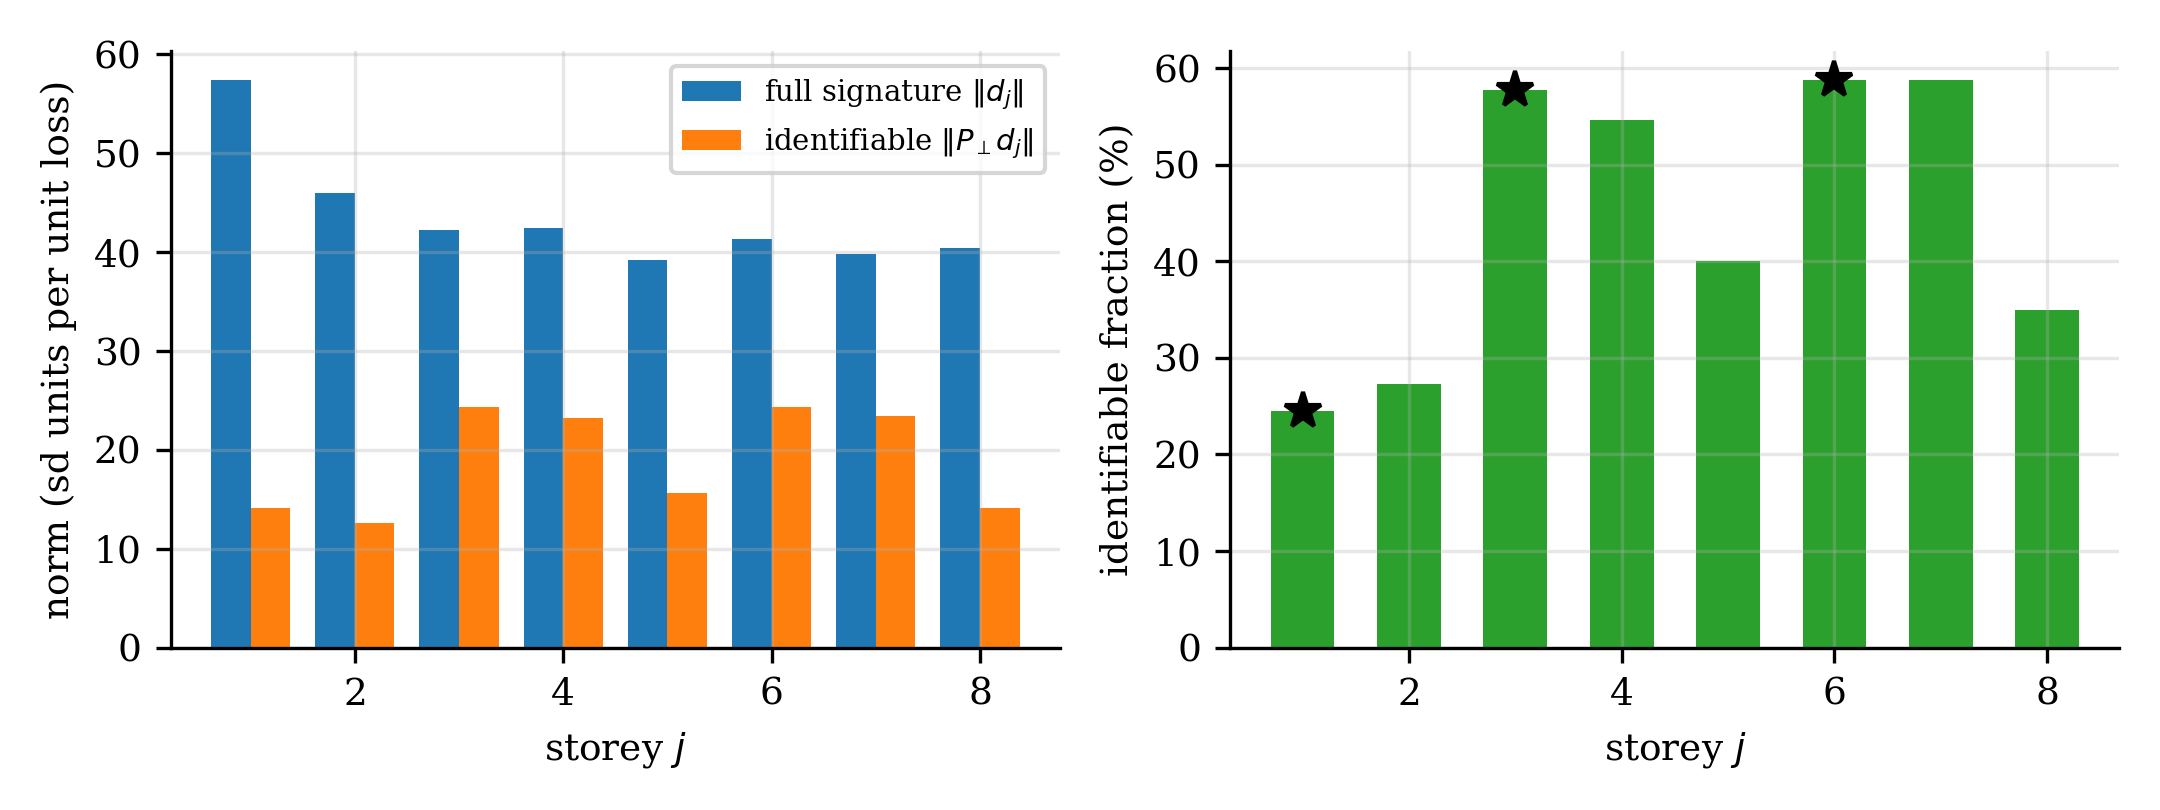
\includegraphics[width=\textwidth]{fig_detectability.png}
\caption{Physics-derived detectability map. Left: full signature norm and the part surviving projection out of the nuisance subspace. Right: identifiable fraction by storey; stars mark the storeys used in the damage scenarios.}
\label{fig:detect}
\end{figure}

\subsubsection{Commissioning window: a structural prerequisite}

Table~\ref{tab:burn} reports a sweep over commissioning length. The results are unforgiving. With 30 or 60 days of commissioning the monitor is invalid: false-alarm probabilities of 0.24 and 0.25 for PHASE, and 0.73 and 0.63 for the black-box variant. The mechanism is extrapolation. The bias discount $\hat\delta$ measures misspecification inside the observed covariate envelope, and a monitor commissioned in one season spends the rest of the year outside it. At 120 days validity returns (0.01) but detection collapses to zero, because the enlarged $\hat\delta$ consumes all the evidence a 5\% signal can generate. Only with a full seasonal cycle do validity and power coexist.

\begin{table}[t]
\centering
\small
\caption{Commissioning-window sweep: false-alarm probability on undamaged records and detection of 5\% loss at storey 3, from 100 records per cell. Coverage is the fraction of monitoring epochs whose covariates fall inside the commissioning envelope.}
\label{tab:burn}
\begin{tabular}{lccccccc}
\toprule
& & & \multicolumn{2}{c}{PHASE} & \multicolumn{2}{c}{PHASE-BB} & PHASE-E \\
\cmidrule(lr){4-5}\cmidrule(lr){6-7}\cmidrule(lr){8-8}
Window & Coverage & $\hat\delta$ & FWFA & Detection & FWFA & Detection & FWFA \\
\midrule
30 days  & 0.44 & 0.076 & 0.24 & 0.23 & 0.73 & 0.05 & 0.11 \\
60 days  & 0.45 & 0.074 & 0.25 & 0.09 & 0.63 & 0.05 & 0.16 \\
120 days & 0.75 & 0.119 & 0.01 & 0.00 & 0.09 & 0.00 & 0.04 \\
365 days & 0.98 & 0.020 & 0.00 & 1.00 & 0.00 & 1.00 & 0.00 \\
\bottomrule
\end{tabular}
\end{table}

Within this bleak picture, the physics-structured surrogate degrades markedly more gracefully than the black-box alternative -- a factor of three in false-alarm probability at 30 days -- which is the clearest evidence in our study for the value of physics in the nuisance model. Envelope gating, which suspends betting outside the commissioning envelope, roughly halves the false-alarm probability at 30 days but monitors only 44\% of epochs and does not restore validity. This is a negative result with a constructive implication, taken up in Section~6.

Notably, once a full seasonal cycle is available, the black-box surrogate matches the physics-structured one on both validity and delay (Table~\ref{tab:delay}). With 1{,}460 epochs of commissioning data there is ample information to fit 30 parameters, and the advantage of physical structure is largely exhausted. Physics buys data efficiency and graceful degradation, not unconditional superiority, and we think it is more useful to say so than to select the comparison that flatters the method.

\begin{figure}[t]
\centering
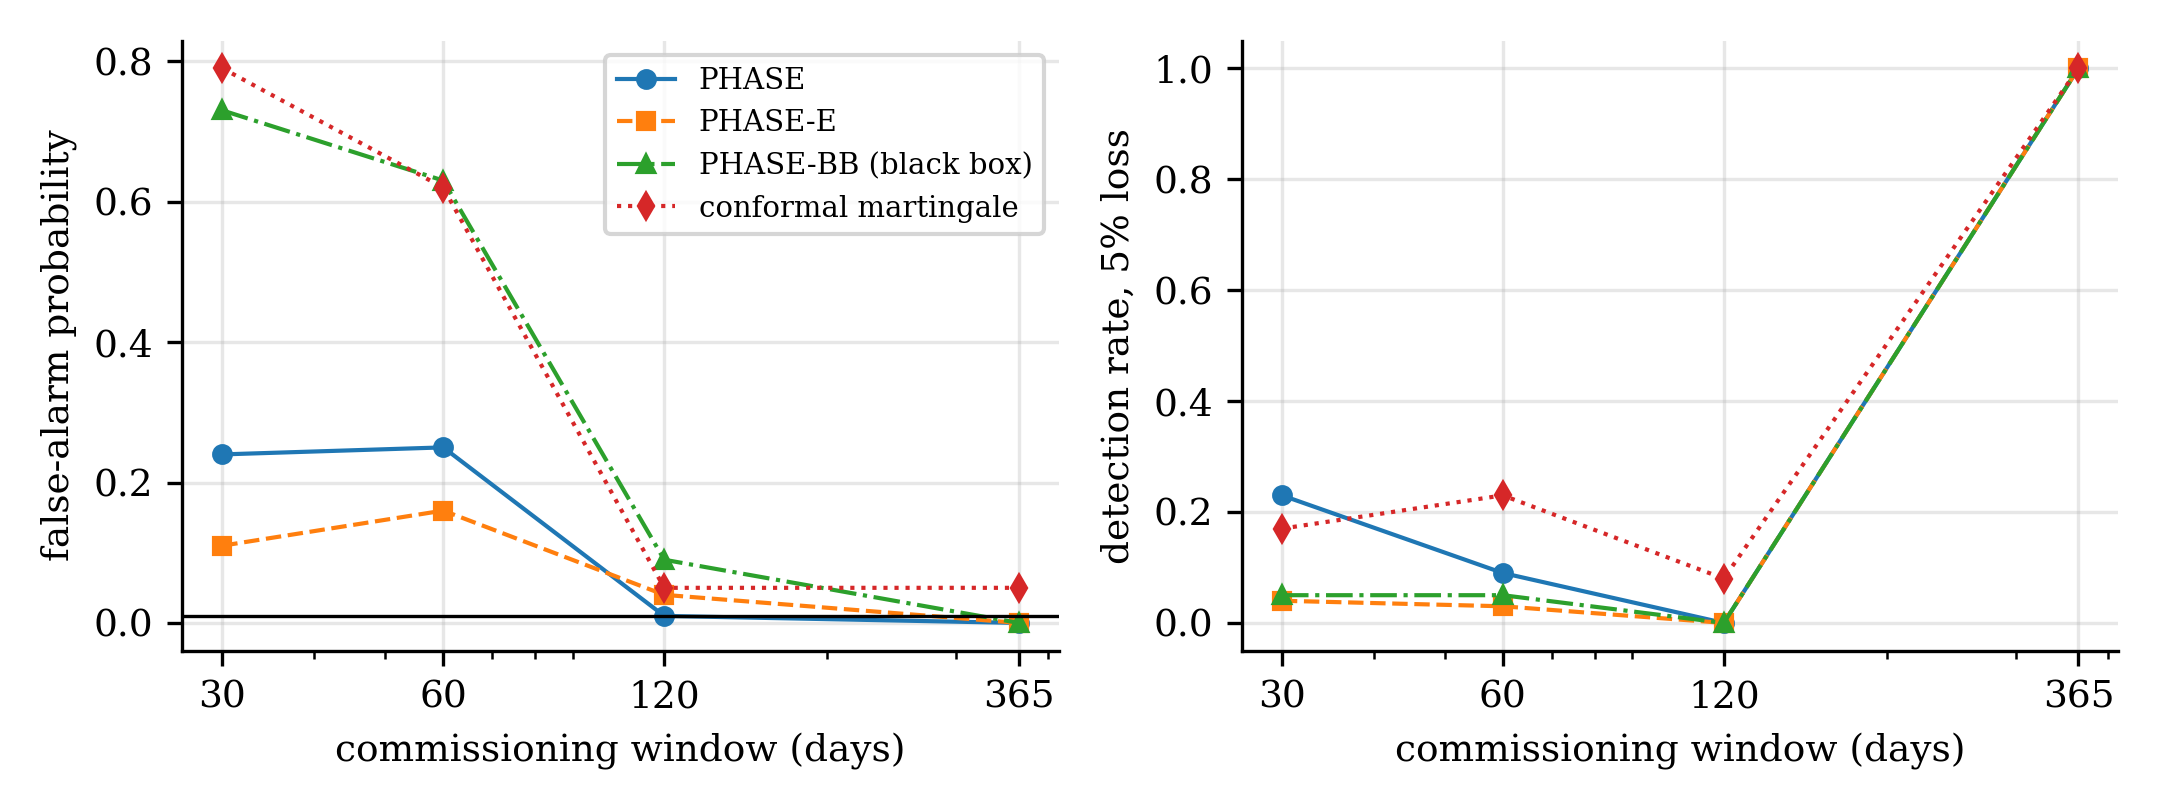
\includegraphics[width=\textwidth]{fig_commissioning.png}
\caption{Effect of commissioning-window length on false-alarm probability (left) and on detection of 5\% stiffness loss (right). Validity and power coexist only when commissioning spans the operational envelope.}
\label{fig:comm}
\end{figure}

\subsubsection{Operational and environmental translation}

The guarantee in Proposition~\ref{prop:valid} converts into an unusually clean operational statement. It is not a rate per epoch or per year but a bound over the monitoring life: across a fleet of instrumented structures, at most a proportion $\alpha$ will ever raise a false alarm, however long they are monitored. At $\alpha=0.01$, a portfolio of 500 monitored buildings expects at most five spurious inspection triggers in total, not per year.

The contrast with threshold-based practice is stark. A $3\sigma$ chart that is reset after each investigation and whose first alarm arrives after a median of two days implies inspection triggers of order $10^2$ per structure-year. Table~\ref{tab:carbon} translates the difference using a user-supplied mobilisation factor; we deliberately avoid asserting a carbon value for an inspection, since it depends on crew travel, access equipment and structure type, and asset owners should substitute locally derived factors. The arithmetic is linear and the conclusion is insensitive to the factor chosen: the avoided burden is dominated by the alarm rate, which differs across monitors by four orders of magnitude.

\begin{table}[t]
\centering
\small
\caption{Illustrative annual inspection burden for a portfolio of 500 monitored structures. Alarm rates for the $3\sigma$ chart are an order-of-magnitude implication of its median two-day time to first alarm under reset; the PHASE figure is the bound of Proposition~\ref{prop:valid} spread over an assumed 20-year monitoring life. Mobilisation factors are placeholders to be replaced with locally derived values.}
\label{tab:carbon}
\begin{tabular}{lccc}
\toprule
& $3\sigma$ chart & Calibrated chart & PHASE \\
\midrule
Spurious triggers per structure-year & $\sim$180 & $\sim$0.007 & $\le$0.0005 \\
Portfolio triggers per year & $\sim$90{,}000 & $\sim$3.5 & $\le$0.25 \\
\midrule
tCO\textsubscript{2}e/yr at 50\,kg per mobilisation & 4{,}500 & 0.18 & 0.01 \\
tCO\textsubscript{2}e/yr at 150\,kg per mobilisation & 13{,}500 & 0.53 & 0.04 \\
tCO\textsubscript{2}e/yr at 400\,kg per mobilisation & 36{,}000 & 1.4 & 0.10 \\
\bottomrule
\end{tabular}
\end{table}

The comparison with the calibrated chart is the honest one, and it is not primarily about carbon: both raise few alarms, but the calibrated chart achieves this by being unable to detect damage at all in our experiments, whereas PHASE detects 5\% stiffness loss in every record within two months. The environmental case for anytime-valid monitoring rests less on avoided inspections than on preserving the detection capability that makes early, repair-scale intervention possible.

\section{Application to the Z24 bridge}

The simulation study above is controlled but synthetic. This section applies PHASE to real measurements from the Z24 progressive damage test, the canonical benchmark in vibration-based SHM \citep{peeters2001z24}, in which a three-span prestressed concrete highway overpass near Koppigen, Switzerland, was subjected to a documented sequence of structural interventions before demolition in 1998; the test programme is described in detail by \citet{reynders2009z24}.

\subsection{Data and modal feature extraction}

We use the released ambient-vibration records for the first ten test states: two undamaged reference measurements (4 and 9 August 1998), progressive lowering of the Koppigen pier by 20, 40, 80 and 95\,mm, a foundation tilt, a third reference measurement taken after the settlement had been reversed and the pier lifted back, and concrete spalling at the soffit over 12 and 24\,m$^2$. Accelerations were sampled at 100\,Hz in nine instrument setups per state; we use only the five permanently installed reference accelerometers, which are common to every setup and therefore free of the roving-sensor differences between setups. Both released measurement modalities are analysed: ambient vibration, driven by traffic and wind, and forced vibration, driven by shakers. The forced records have a better signal-to-noise ratio and give within-state coefficients of variation of 0.24--0.97\% against 0.35--1.4\% for the ambient records, so they serve as an independent check that the conclusions are not artefacts of one excitation type.


% ---------------------------------------------------------------------------
% If photographs of the Z24 bridge are cleared for re-use (Reynders and
% De Roeck, 2009; DOI 10.1002/9780470061626.shm165), uncomment the two
% minipages below, place the image files alongside main.tex, and add the
% permission wording required by the rights holder to the caption.
%
% \begin{minipage}[b]{0.48\textwidth}
% \centering
% \includegraphics[width=\textwidth]{fig_z24_photo.png}\\[2pt]{\small (a)}
% \end{minipage}\hfill
% \begin{minipage}[b]{0.48\textwidth}
% \centering
% \includegraphics[width=\textwidth]{fig_z24_rig.png}\\[2pt]{\small (b)}
% \end{minipage}
% \vspace{6pt}
% ---------------------------------------------------------------------------
\begin{figure}[t]
\centering
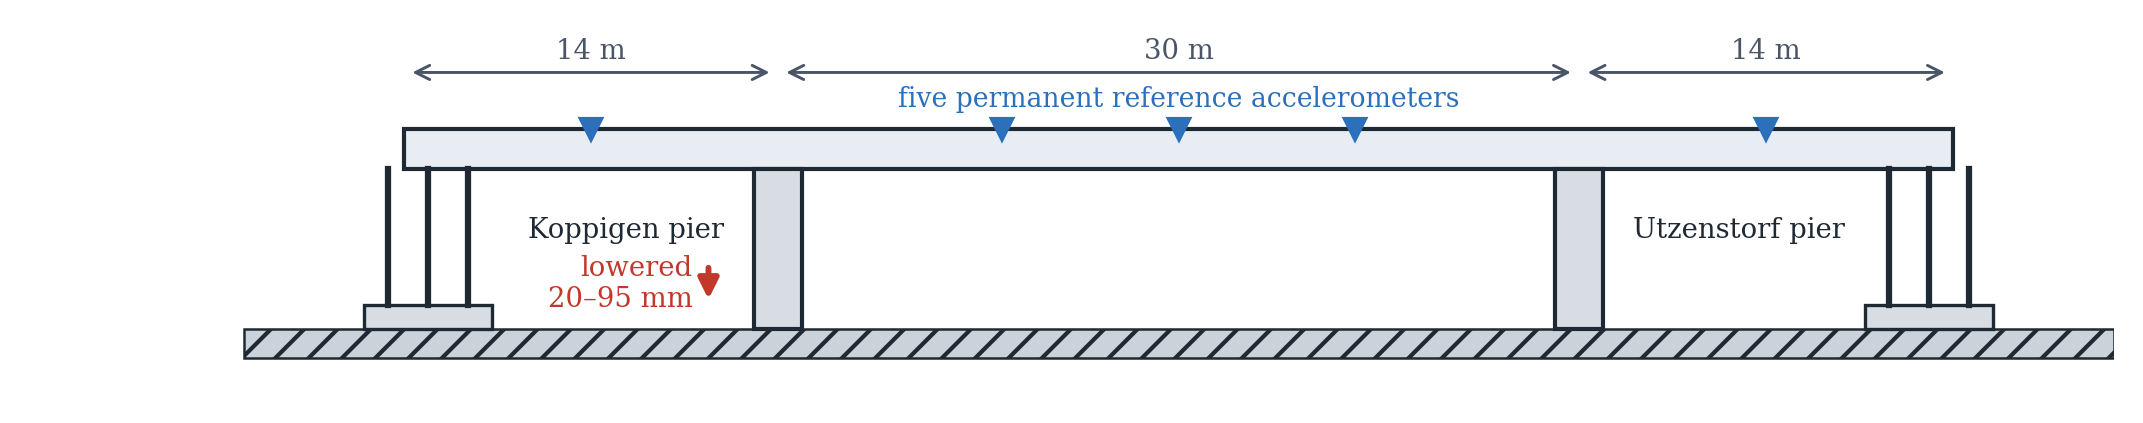
\includegraphics[width=0.92\textwidth]{fig_bridge.png}
\caption{Schematic elevation of the Z24 bridge: a three-span prestressed concrete box-girder overpass, with the two central piers stiffly connected to the girder and column triplets at the abutments. Progressive damage was introduced by lowering the Koppigen pier in four stages, producing the settlement sequence analysed in experiment R2; the lowering was later reversed, which experiment R3 analyses. Accelerometer positions are indicative only. Drawing by the authors; dimensions follow the published description of the structure \citep{peeters2001z24,reynders2009z24}.}
\label{fig:bridge}
\end{figure}

Each record is divided into non-overlapping windows of 8{,}192 samples (81.9\,s), each treated as one monitoring epoch. For each epoch the cross-power spectral density matrix of the five reference channels is formed by Welch's method and its first singular value taken, that is, frequency domain decomposition; three natural frequencies are then peak-picked in fixed bands with parabolic interpolation. This yields 690 ambient and 711 forced epochs across the ten states. The three tracked modes lie near 3.87, 9.82 and 12.7\,Hz and have within-state coefficients of variation of 0.35\%, 0.75\% and 1.4\%; other candidate bands were discarded because the automatic picker could not track them consistently across all ten states, and this restriction to $m=3$ features is a limitation of the analysis rather than of the data.

Figure~\ref{fig:bridge} shows the structure and the location of the intervention. Figure~\ref{fig:z24}(left) shows the resulting state means. The physics is clearly visible: all three frequencies fall monotonically through the settlement sequence, by 4.9\%, 1.3\% and 4.0\% respectively at 95\,mm, and all three recover when the settlement is reversed.

\subsection{What this dataset can and cannot test}

Two features of the released data constrain what may be concluded, and we state them before reporting results. First, no environmental covariate accompanies the ambient-vibration files, so the physics-structured surrogate of Section~3.3 degenerates to a predictable running intercept and the identifiability analysis cannot be exercised; correspondingly, the damage cone is instantiated at its coarsest physically justified level, namely that stiffness loss cannot raise a natural frequency, so the admissible set is the non-positive orthant in standardised log-frequency space. Localisation is not attempted, as no calibrated finite element model of the bridge is available to us.

Second, and more consequentially, each state was measured on a different day. The two undamaged reference measurements, taken five days apart, differ by 0.9\%, 1.4\% and 0.3\% in the three tracked modes, which is two to four times the within-state scatter. Test-day effects are therefore of the same order as the damage signatures, and no monitor can attribute a change to damage rather than to environment without a covariate. Because epochs within a state are exchangeable, all results below are reported over 200 random orderings of the epochs within each block, giving Monte Carlo standard errors on alarm rates.

\subsection{Results}

Table~\ref{tab:z24} reports six experiments.

\begin{table}[t]
\centering
\scriptsize
\setlength{\tabcolsep}{2.6pt}
\caption{Z24 bridge: alarm rate over 200 random epoch orderings; median alarm epoch in parentheses for R2, where timing distinguishes the methods. Nominal level $\alpha=0.01$; standard errors at most 0.035. PH-$\Omega$ is the cone-free ablation, CTM the conformal test martingale, MSD the Mahalanobis novelty index. EWMA and Shiryaev--Roberts, omitted for space, behave like CUSUM. Without replicate healthy campaigns, all thresholds here are calibrated on the commissioning window alone, as a practitioner would have to do.}
\label{tab:z24}
\begin{tabular}{llcccccccc}
\toprule
& Commissioning $\to$ monitored state & PHASE & PH-$\Omega$ & CTM & CUSUM & 3$\sigma$ & $\chi^2$ & PCA & MSD \\
\midrule
\multicolumn{10}{l}{\textit{ambient vibration (690 epochs)}}\\
R1a & ref 1 $\to$ ref 2 (new day) & 1.00 & 1.00 & 1.00 & 1.00 & 1.00 & 1.00 & 0.97 & 0.90 \\
R1b & ref 1+2 $\to$ held-out ref. & \textbf{0.00} & \textbf{0.00} & 0.01 & 0.86 & 0.07 & 0.14 & \textbf{0.00} & 0.68 \\
R2  & ref 1+2 $\to$ settlement 20--95 mm & 1.00 (72) & 1.00 (119) & 1.00 (76) & 1.00 & 1.00 & 1.00 & 1.00 (105) & 1.00 (143) \\
R3  & 95 mm $\to$ reversed (recovery) & \textbf{0.00} & 1.00 & \textbf{0.00} & \textbf{0.00} & 1.00 & 1.00 & 1.00 & 1.00 \\
R4  & ref 1+2 $\to$ spalling 12, 24 m$^2$ & 1.00 & 1.00 & 1.00 & 1.00 & 1.00 & 1.00 & 0.53 & 0.22 \\
R5  & ref 1+2 $\to$ reference 3 (new day) & 1.00 & 1.00 & 1.00 & 1.00 & 1.00 & 1.00 & 0.52 & 0.18 \\
\midrule
\multicolumn{10}{l}{\textit{forced vibration (711 epochs)}}\\
R1a & ref 1 $\to$ ref 2 (new day) & 1.00 & 1.00 & 1.00 & 1.00 & 1.00 & 1.00 & 1.00 & 1.00 \\
R1b & ref 1+2 $\to$ held-out ref. & \textbf{0.00} & \textbf{0.00} & 0.01 & 0.86 & 0.42 & 0.35 & \textbf{0.00} & \textbf{0.00} \\
R2  & ref 1+2 $\to$ settlement 20--95 mm & 1.00 (29) & 1.00 (103) & 1.00 (31) & 1.00 & 1.00 & 1.00 & 1.00 (144) & 1.00 (144) \\
R3  & 95 mm $\to$ reversed (recovery) & \textbf{0.00} & 1.00 & \textbf{0.00} & \textbf{0.00} & 1.00 & 1.00 & 1.00 & 1.00 \\
R4  & ref 1+2 $\to$ spalling 12, 24 m$^2$ & 1.00 & 1.00 & 1.00 & 1.00 & 1.00 & 1.00 & 1.00 & 0.87 \\
R5  & ref 1+2 $\to$ reference 3 (new day) & 1.00 & 1.00 & 1.00 & 1.00 & 0.84 & 0.95 & 0.91 & 0.14 \\
\bottomrule
\end{tabular}
\end{table}

\paragraph{The commissioning envelope, confirmed on real data.} R1a commissions the monitor on the first reference measurement and then monitors the second, five days later, with no damage in between. Every method, PHASE included, alarms in every ordering under both excitation types. The estimated bias discount, $\hat\delta=0.13$--$0.14$, was calibrated within a single test day and does not cover between-day variation. R1b repeats the exercise with the commissioning window pooled across both reference days and monitoring held-out reference epochs: PHASE, its omnibus variant and the PCA chart then alarm in none of 200 orderings, the conformal martingale in 1\%, while the repeated $\chi^2$ test alarms in 14\% of ambient and 35\% of forced orderings, and CUSUM and Shiryaev--Roberts -- whose thresholds a practitioner without replicate healthy campaigns must calibrate on the commissioning window -- alarm in 86\% and 83\%. The simulation finding of Section~4.2.6, that anytime-valid monitoring requires a commissioning window spanning the operational envelope and is actively misleading otherwise, thus reproduces on real measurements in both modalities.

\paragraph{Directional discrimination, confirmed on real data.} R3 is the real-data counterpart of the benign stiffening experiment. Commissioning on the 95\,mm settled state and then monitoring the state after the settlement had been reversed, PHASE alarmed in none of 200 orderings while the otherwise identical omnibus variant alarmed in all of them, at a median of 14 epochs. The $3\sigma$ chart, the repeated $\chi^2$ test, the PCA chart and the Mahalanobis index also alarmed in every ordering; the result is identical under forced excitation. The bridge really did change, and substantially: all three frequencies rose, by 4.6\%, 0.9\% and 2.7\%. A damage detector should not report damage when a structure recovers stiffness, and the physics-derived sign restriction is what supplies that discrimination. The conformal martingale, CUSUM, Shiryaev--Roberts and EWMA also stay silent here, but they consume the same cone score, so their immunity is inherited from the physics rather than earned by their own machinery. Because the restriction is directional, this conclusion is immune to the attribution difficulty discussed below: whatever caused the frequencies to rise, damage did not.

\paragraph{Detection, with an attribution caveat.} In R2 the monitor is commissioned on both reference days and then sees the settlement sequence. PHASE alarms in every ordering, at a median of 72 epochs under ambient excitation and 29 under forced excitation, where the lower identification scatter roughly halves the delay. The omnibus variant alarms considerably later in both cases, at 119 and 103 epochs, and the two data-normalisation charts later still, at 105--144. The ordering is what the cone predicts, and the margin is substantial and consistent across modalities. It would be tempting to read the R2 alarm as damage detection, but R5 forbids it: monitoring the third reference measurement, taken on yet another day after the settlement was reversed, also produces an alarm in every ordering for every sequential method. That state is nominally undamaged, though it is documented as not identical to the original condition, the pier support having been altered by the lifting operation. With only two reference days in the commissioning envelope, any subsequent test day exceeds it. We therefore report R2 and R4 as demonstrating that PHASE responds to real structural change earlier than an omnibus detector, and explicitly not as evidence that it separates damage from environment on this dataset. That separation requires the covariate stream that the Z24 release does not include.

\begin{figure}[t]
\centering
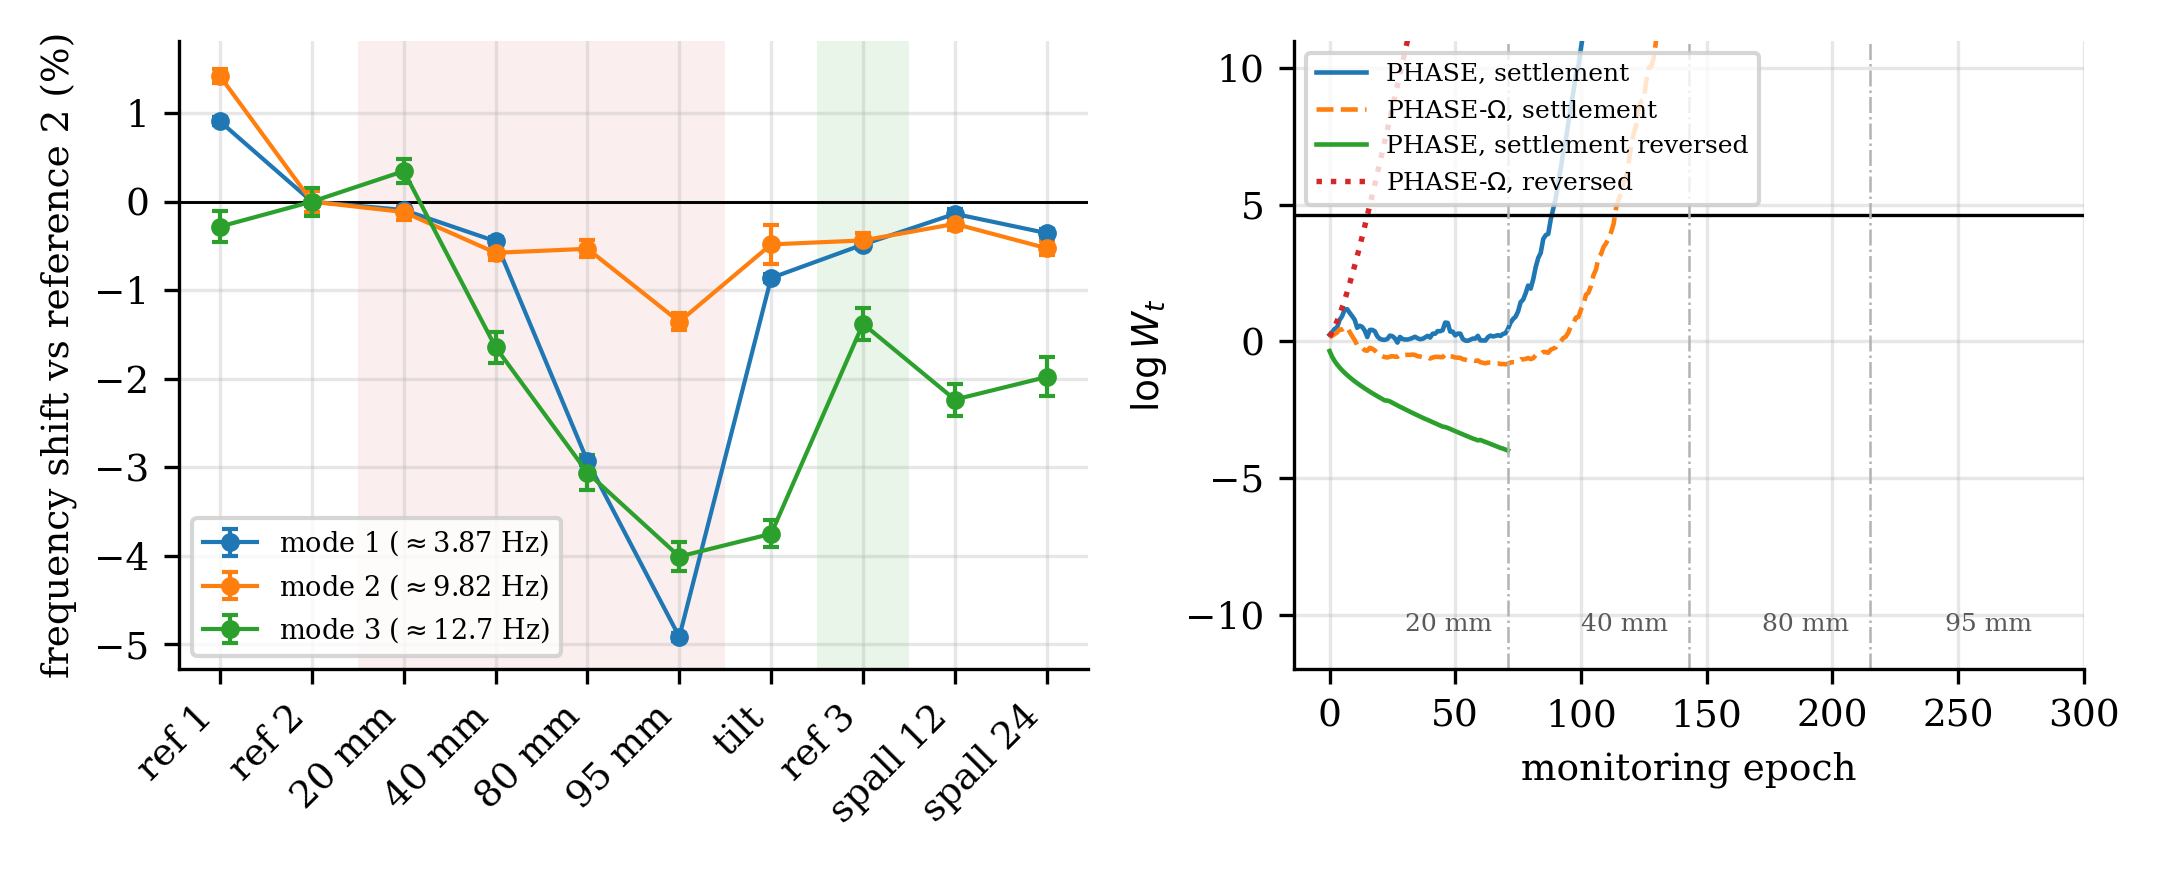
\includegraphics[width=\textwidth]{fig_z24.png}
\caption{Z24 bridge. Left: mean shift of the three tracked natural frequencies in each structural state relative to the second reference measurement, with standard errors; shading marks the settlement sequence (red) and the state after the settlement was reversed (green). Right: accumulated log-evidence for PHASE and the omnibus variant under the settlement sequence and under the reversal, with the alarm threshold.}
\label{fig:z24}
\end{figure}

\subsection{What the real-data study adds}

Three claims of the paper survive contact with real measurements. The commissioning-envelope requirement is confirmed, and confirmed as a failure mode of PHASE and not only of its competitors. The value of restricting the alternative to physically admissible directions is confirmed in the cleanest possible form, on a genuine structural change of known sign. And the evidence accumulated by the cone-restricted process crosses the alarm threshold earlier than that of the omnibus process on a real damage sequence. Both conclusions hold under ambient and forced excitation, so neither is an artefact of one excitation type. What the dataset cannot support, and what we therefore do not claim, is calibrated separation of damage from environmental variation: that would require a monitoring campaign with a synchronous covariate record, of which the Z24 long-term monitoring series and the KW51 campaign are the obvious candidates for future work.

\section{Discussion and conclusions}

\subsection{Implications for practice}

Three practical implications follow. First, alarm governance becomes a budget rather than a tuning exercise. An asset owner can state that at most 1\% of monitored structures will ever raise a false alarm and hold the monitoring system to that commitment, which is a specification that can be written into a contract. Because the guarantee is uniform over stopping rules, operators may also watch the evidence process continuously and act on a rising trajectory before the threshold is crossed, without the informal peeking that invalidates conventional tests.

Second, the detectability map belongs in the design phase. It is computed from the finite element model and the expected identification scatter, before installation, and states which substructures a proposed sensor and mode configuration can support claims about. In our eight-storey frame, moving from four to six identified modes raised the identifiable fraction at storeys 1 and 8 from 0.034 and 0.064 to 0.245 and 0.349, converting effectively blind substructures into monitorable ones. This is a concrete, physics-derived criterion for instrumentation planning, and it integrates naturally with BIM-based asset models where the finite element model and sensor layout already coexist.

Third, the commissioning requirement should be treated as a design constraint rather than a nuisance. Our results indicate that a monitoring system commissioned over a single season is not merely less powerful but positively misleading. Where waiting a full year is unacceptable, the natural remedy is exactly the one this special issue is concerned with: use the calibrated digital twin to \emph{synthesise} the operational envelope, generating reference-condition modal responses across temperatures and load states that have not yet been observed, and calibrate $\hat\delta$ against simulated rather than measured excursions. This substitutes model risk for extrapolation risk, and quantifying that trade-off is a natural next step.

\subsection{Sustainability implications}

The sustainability case for instrumented infrastructure rests on the claim that continuous monitoring enables condition-based intervention: repairs made early, at small scale, in place of replacement. That claim depends on alarms being both trusted and timely. Our results indicate that conventional practice can satisfy neither simultaneously -- naive charts alarm constantly, and charts calibrated to stop alarming stop detecting -- while an anytime-valid rule can. The relevant environmental benefit is therefore not primarily the avoided carbon of unnecessary inspections, real though that is, but the preservation of the embodied carbon in structures that are repaired rather than replaced because deterioration was detected while it was still small. Reviews of AI in the built environment tend to locate sustainability gains in energy optimisation and material efficiency \citep{bibri2025aidt}; the gain argued here is of a different kind, residing in the trustworthiness of the decisions a monitoring system supports. This connects to SDG 9 through resilient infrastructure, SDG 11 through the safe operation of the existing building stock, and SDG 13 through the emissions avoided by extending service life.

There is a further, less obvious implication for equity. The commissioning result implies that rigorous monitoring requires patience rather than expensive hardware, and the physics-informed surrogate delivers usable behaviour from many fewer parameters than a black-box alternative. Both features favour deployment in rapidly urbanising contexts where instrumentation budgets are constrained but the building stock is young and its deterioration curve has not yet been characterised.

\subsection{Limitations}

The controlled evidence here is simulation-based and the real-data study is limited in the ways set out in Section~5.2: three tracked modes, no covariate record, no localisation, and states measured on different days so that detection cannot be attributed to damage rather than environment. The generator was constructed to be adversarial in specific ways -- unmodelled thermal lag and gradients, heavy-tailed identification noise, an imperfect load proxy -- but a shear frame is a simple structure, real EOV includes effects we did not model such as humidity, wind and freeze--thaw stiffening, and real modal identification produces mode-mismatching and dropouts that we did not simulate. The Z24 progressive damage test exercises the directional and commissioning claims on real measurements but cannot exercise the identifiability analysis; a campaign with synchronous temperature, such as the Z24 long-term monitoring series or the KW51 retrofitting campaign, is the necessary next step.

Several limitations are methodological. Only frequencies are used; mode shapes and their derivatives carry localisation information that the cone construction could exploit directly. The null \eqref{eq:null} is stated as a conditional mean bound and made true by the surrogate rather than assumed of the physics, which is honest but places weight on $\hat\delta$; that estimate is itself a two-standard-error bound from a finite commissioning sample, and our commissioning sweep shows exactly how it fails when the envelope is not covered. The detection delays reported are two to three times those of an oracle CUSUM, which is the price of the anytime guarantee, and for a structure monitored under a genuinely fixed horizon by an analyst who never peeks, the oracle procedure would be preferable. Finally, the localisation index is a heuristic accumulator rather than a calibrated estimator; giving localisation claims their own anytime-valid guarantee via e-value based false discovery rate control across zones is a clear extension.

\subsection{Conclusions}

Structural health monitoring systems make thousands of decisions per year using rules designed for one. This paper has shown that the resulting false-alarm probability is not a small correction -- a $3\sigma$ chart alarmed on every undamaged structure within days -- and that the usual remedy of raising thresholds trades the problem for a worse one, since a chart calibrated to control error over a monitoring year detected no 5\% damage at all in our experiments.

PHASE addresses this by replacing the threshold with a betting e-process whose guarantee holds at every instant of an unbounded campaign, and by using eigenvalue perturbation in four distinct roles: constraining the nuisance surrogate, restricting the alternative to a polyhedral damage cone, determining which stiffness-loss patterns are identifiable at all, and protecting identifiable damage from online adaptation. Across 2{,}700 simulated records it raised no false alarm on undamaged structures at either one- or three-year horizons, detected 5\% single-storey stiffness loss in every record within a median of 59 days, localised it correctly wherever the signature was identifiable, and remained silent under a benign stiffening event that an otherwise identical omnibus detector flagged in every record.

On real measurements from the Z24 bridge the two claims that the data can test both hold: a monitor commissioned within a single test day false-alarms on the next undamaged day, whereas one commissioned across both reference days does not; and when the pier settlement was reversed and the bridge recovered stiffness, PHASE stayed silent in all 200 epoch orderings while every omnibus detector reported damage in all of them.

Two findings qualify the method and, we believe, matter more than the headline comparisons. Uniform stiffness loss is confounded with a temperature change as a matter of structure, not of statistical power, so a monitor should state which substructures it can and cannot speak about. And calibrated monitoring requires a commissioning window spanning the operational envelope; below that, monitors are not conservative but actively misleading. Both limitations are consequences of the physics, and both are visible only because the physics was carried into the inference rather than left in the surrogate. The Z24 study adds a third: without a synchronous environmental covariate, no monitor can attribute a change to damage, and reporting detection rates on such data risks crediting the detector for the calendar.

\newpage
\bibliography{refs}

\newpage
\appendix
\section*{Appendix: Proofs}
\addcontentsline{toc}{section}{Appendix}

\paragraph{Proposition~\ref{prop:ident}.}
By \eqref{eq:shift} the standardised signature of a loss pattern $\rho$ is $-D^{-1}S\rho$. A uniform modulus change of relative size $\epsilon$ produces $-\tfrac12\epsilon D^{-1}\kappa$ and a relative added mass $\zeta$ produces $-\tfrac12\zeta D^{-1}\eta$, so the set of signatures attainable by the nuisance is exactly $\mathcal{N}$. Hence $\rho$ is confounded if and only if $D^{-1}S\rho\in\mathcal{N}$, and the component of the signature carrying information not attainable by the nuisance is $P_\perp D^{-1}S\rho$. For $\rho=\rho_0\mathbf{1}$, \eqref{eq:rowsum} gives $S\mathbf{1}=\mathbf{1}=\kappa$, so the signature is $-\rho_0 D^{-1}\kappa\in\mathcal{N}$ and is confounded for every $\rho_0$. If $m\le2$ then generically $\mathcal{N}=\R^m$ and $P_\perp=0$, so no pattern is identifiable. \hfill$\square$

\paragraph{Proposition~\ref{prop:poly}.}
The first claim holds because each $v_k\in\Cone$ has unit norm and $\|\Pi_\Cone(r)\|=\sup_{v\in\Cone,\|v\|\le1}\langle v,r\rangle$. For the second, let $v^\star$ attain the supremum and let $v_k$ satisfy $\angle(v_k,v^\star)\le\gamma$, so $\|v_k-v^\star\|=2\sin(\gamma/2)$. Then by Cauchy--Schwarz $\langle v_k,r\rangle=\langle v^\star,r\rangle+\langle v_k-v^\star,r\rangle\ge\|\Pi_\Cone(r)\|-2\sin(\gamma/2)\|r\|$. Monotonicity is immediate since enlarging $V$ enlarges the set over which the maximum is taken. \hfill$\square$

\paragraph{Proposition~\ref{prop:valid}.}
Fix $\lambda\in[0,1/\mu_0)$. Since $X_t\in[0,1]$, the factor $1+\lambda(X_t-\mu_0)\ge1-\lambda\mu_0>0$, so $W^\lambda_t\ge0$. The bet $\lambda$ is deterministic and $\mu_0$ is an $\F_0$-measurable constant, so
$\E[W^\lambda_t\mid\F_{t-1}]=W^\lambda_{t-1}\big(1+\lambda(\E[X_t\mid\F_{t-1}]-\mu_0)\big)\le W^\lambda_{t-1}$
by \eqref{eq:null} and $\lambda\ge0$. Thus each $W^\lambda$ is a non-negative supermartingale with initial value one, and so is the finite mixture $W_t$, convex combinations of supermartingales being supermartingales. Ville's inequality gives $\Prob(\exists t: W_t\ge1/\alpha)\le\E[W_{t_0}]\alpha=\alpha$. Nothing in the argument uses independence across epochs, the marginal law of $X_t$, or the accuracy of $\hat\beta_{t-1}$; only predictability of the bets and of the plug-in, which holds by construction, and the conditional mean bound \eqref{eq:null}. The same argument covers predictable bet sequences $\lambda_t$, since $\lambda_t$ then factors out of the conditional expectation. \hfill$\square$

\paragraph{Proposition~\ref{prop:delta}.}
Under the relaxed null, $\E[1+\lambda(X_t-\mu_0)\mid\F_{t-1}]\le1+\lambda\delta$, so dividing the increment by the deterministic factor $1+\lambda\delta$ restores the supermartingale property:
$\E[\widetilde W^\lambda_t\mid\F_{t-1}]\le\widetilde W^\lambda_{t-1}$. Ville's inequality applies as before. \hfill$\square$

\paragraph{Proposition~\ref{prop:delay}.}
Write $Z_s=\log(1+\lambda(X_s-\mu_0))-\log(1+\lambda\delta)$ and $\bar g=g(\lambda)-\log(1+\lambda\delta)>0$. Then $\sum_{s\le t}(Z_s-\E[Z_s\mid\F_{s-1}])$ is a martingale with increments bounded by $B$, and $\E[Z_s\mid\F_{s-1}]\ge\bar g$ after $t^\star$. The mixture satisfies $\log W_t\ge-\log|\Lambda|+\log\widetilde W^\lambda_t$, so the alarm occurs no later than the first $t$ with $\log\widetilde W^\lambda_t\ge\log(1/\alpha)+\log|\Lambda|$. Applying the optional stopping theorem to the stopped martingale and using Wald's identity gives
$\bar g\,\E[\tau-t^\star]\ \ge\ \log(1/\alpha)+\log|\Lambda|-(\log W_{t^\star})^{-}-B$,
which rearranges to \eqref{eq:delay}. The condition $\bar g>0$ is exactly the requirement that the damage generate evidence faster than the bias discount consumes it. \hfill$\square$

\end{document}
